\documentclass{article}
\usepackage[latin1]{inputenc}
\usepackage[T1]{fontenc}
\usepackage{times}
\usepackage{url}
\usepackage{amsmath}
\usepackage{alltt}
\usepackage[final]{graphicx}

\begin{document}
\title{\textsc{melting} - nearest-neighbor computation of nucleic acid hybridation}
\author{Marine Dumousseau \and Nicolas Le Nov\`ere \\
  \texttt{lenov@ebi.ac.uk}}
\date{August 2009}
\maketitle

\newpage
\nocite{*}

\section{Synopsis}
The nearest-neighbor approach is based on the fact that the helix-coil
transition works as a zipper. After an initial attachment, the hybridisation
propagates laterally.
The hybridization process depends on the adjacent nucleotides on each strand (the Crick's pairs).  
Two duplexes with the same base pairs could have different stabilities, and on the contrary, two 
duplexes with different sequences but identical sets of Crick's pairs will have the same
thermodynamics properties (see Sugimoto et al. 1994).
See Wetmur J.G (1991) and Santalucia (1998) for deep reviews on the nucleic acid hybridization
and on the different set of nearest-neighbor parameters.
 
\section{Description }

\textsc{melting} computes, for a nucleic acid duplex, the enthalpy and the
entropy of the helix-coil transition, and then its melting temperature. Four
types of hybridisation are possible: DNA/DNA, DNA/RNA, RNA/RNA and 2-O-Methyl RNA/RNA. The program
uses the method of nearest-neighbors. The set of thermodynamic parameters can be
easely changed, for instance following an experimental breakthrough. Melting is
a free program in both sense of the term. It comes with no cost and it is
open-source. In addition it is coded in Java (1.5) and can be compiled on any
operating system.


If you use \textsc{melting}, please quote

\begin{quote}
  Le Nov\`ere. \textsc{melting}, a free tool to compute the
    melting temperature of nucleic acid duplex. \emph{Bioinformatics}, 17: 1226-1227. 
\end{quote}

\section{Usage}

The options are treated sequentially. If there is a conflict between the value
of two options, the latter normally erases the former.

\subsection{Information about MELTING}
\begin{description}

\item [\textbf{-h}]\mbox{}\\ 
  Displays a short help and quit.
\item [\textbf{-L}]\mbox{}\\ 
  Prints the legal informations and quit. 
\item [\textbf{-V}  ]\mbox{}\\ 
  Displays the version number and quit.  
\item [\textbf{-p}]\mbox{}\\ 
  Return the directory supposed to contain the sets of calorimetric parameters and quit. 
  If the environment variable NN\_PATH is set, it is returned. Otherwise, the value
  defined by default during the compilation is returned.
\end{description}

\subsection{Mandatory options}
\begin{description}

\item [\textbf{-S} \textit{sequence}  ]\mbox{}\\ 
  Sequence of one strand of the nucleic 
  acid duplex, entered 5' to 3'. \textbf{Important:} 
  Uridine and thymidine are not considered as identical. The bases can be upper or lowercase.
\item [\textbf{-C} \textit{complementary\_sequence}] \mbox{}\\
  Enters the complementary sequence, from 3' to 5'. This option is mandatory if
  there are mismatches, inosine(s) or hydroxyadenine(s) between the two strands. If it is not used, the program
  will compute it as the complement of the sequence entered with the option \textbf{-S}. In case of self complementary sequences,
  The program can automatically detect the symmetry and deduce the complementary even though there is (are) dangling
  end(s) and it is not necessary to write the complementary sequence with the option \textbf{-C}.
  Uridine and thymidine are not considered as identical. The bases can be upper or lowercase.
\item [\textbf{-E} \textit{ion1\_name=x.xxe-xx:ion2\_name=x.xxe-xx:agent1\_name=x.xxe-xx...}] \mbox{}\\
  Enters the different ion (Na, Mg, Tris, K) or agent (dNTP, DMSO, formamide) concentrations. The effect  
  of  ions and denaturing agents on  thermodynamic  stability  of nucleic  acid duplexes is complex,
  and the correcting functions are  at  best rough  approximations. All the concentrations must be positive numeric
  values and in M. There are some exceptions for the DMSO concentrations (in
  \%) and the formamide concentrations
  (in \% or M depending on the used correction method). Be aware, the $[\mbox{Tris}^+]$ is about half of the total tris buffer
  concentration.
  At least one cation concentration is mandatory, the other agents are optional. See the documentation for the concentration 
  limits. It depends on the used correction.
\item [\textbf{-P} \textit{x.xxe-xx}]\mbox{}\\ 
  Concentration of the nucleic acid strand in excess. It must be a strict positive numeric value and it is mandatory. The oligomer
  concentration is in mol/L.
\item [\textbf{-H} \textit{hybridisation\_type}]\mbox{}\\
  Specifies the hybridisation type. Moreover this parameter determines the nature of the sequences entered by the user.
  Possible values are :
  \begin{itemize}
  \item [\textit{dnadna}] : DNA sequence (option \textbf{-S}) and DNA complementary sequence (option \textbf{-C})
  \item [\textit{rnarna}] : RNA sequence (option \textbf{-S}) and RNA complementary sequence (option \textbf{-C})
  \item [\textit{dnarna}] : DNA sequence (option \textbf{-S}) and RNA complementary sequence (option \textbf{-C})
  \item [\textit{rnadna}] : RNA sequence (option \textbf{-S}) and DNA complementary sequence (option \textbf{-C})
  \item [\textit{mrnarna}] : 2-o-methyl RNA sequence (option \textbf{-S}) and RNA complementary sequence (option \textbf{-C})
  \item [\textit{mrnarna}] : RNA sequence (option \textbf{-S}) and 2-o-methyl RNA complementary sequence (option \textbf{-C})
  \end{itemize}
  This option is mandatory to select the default equations and methods to use.
\end{description}

\subsection{General options}
\begin{description}

\item [\textbf{-T} \textit{xxx}  ]\mbox{}\\ 
Size threshold before approximative computation. The nearest-neighbour approach 
will be used by default if the length of the sequence is inferior to this threshold,
otherwise it is the approximative approach which will be used by default.
\item [\textbf{-v}]\mbox{}\\ 
Activates the verbose mode, issuing a lot more information about the current run  (try it once 
to see if you can get something interesting).
\item [\textbf{-nnpath} \textit{folder\_pathway}]\mbox{}\\ 
  Change the default pathway (Data) where to find the default calorimetric tables (thermodynamic parameters).
  The program will look for the file in a directory specified during the installation.
  However, if an environment variable NN\_PATH is defined, melting will search in this one first.
\item [\textbf{-O} \textit{output\_file}]\mbox{}\\ 
  The output is directed to this file instead of the standard output. The name of the file must be specified.
\item [\textbf{-self}]\mbox{}\\
  To precise that the sequence entered with the option \textbf{-S} is self complementary. No complementary sequence is mandatory. 
  The program automatically can detect a self complementary sequence for perfect matching sequences or sequences with dangling ends. 
  In these cases, the option \textbf{-self} is not necessary. Otherwise we need to precise that the sequences are self complementary with this option. 
  examples: 
    
  \begin{verbatim}
  Situation 1 : The sequence ATCGCGAT is self 
                complementary. 
      
  \end{verbatim}
  
  The option \textbf{-self} is not necessary because the program can automatically detect it.
  
  \begin{verbatim}
  Situation 2 : The sequence -TCGCGAT is self 
                complementary with a single 
		dangling end. 
      
  \end{verbatim}
    
  The option \textbf{-self} is not necessary because the program 
  can automatically detect it.
  
  \begin{verbatim}  
  Situation 3 :  If the sequence ATCCCGAT is self 
                 complementary with a single mismatch 
		(C/C)
      
  \end{verbatim}
  		 
  The option \textbf{-self} is necessary to precise the self 
  complementarity because the program can't detect it.
      
 \item [\textbf{-F} \textit{factor}  ]\mbox{}\\
  This is the correction factor used to modulate the effect of the nucleic acid concentration in the computation of the melting temperature. 
  See section ALGORITHM for details. If the sequences are automatically recognized as self complementary sequences or if the option \textbf{-self}
  is used, the factor correction is automatically 1. Otherwise F is 4 if the both strands are present in equivalent amount and 2 if one strand is in excess. 
  The default factor value is 4.
\end{description}

\subsection{Set of thermodynamic parameters and methods (models)}

By default, the approximative mode is used for oligonucleotides longer than 60 bases (the default threshold value), otherwise the nearest 
neighbor model is used. 
\begin{description}

\item [\textbf{-am} \textit{method\_name}]\mbox{}\\ 
  Forces to use a specific approximative formula, based on G+C content. You can use one of the following :
  
  \textsc{DNA duplexes}
    \begin{itemize}
    \item [\textit{ahs01}] (from Ahsen et al. 2001)
    \item [\textit{che93}] (from Marmur, Chester and al. 1962, 1993)
    \item [\textit{che93corr}] (from Ahsen et al. 2001 and from Marmur, Chester and al. 1962, 1993)
    \item [\textit{schdot}] (Marmur-Schildkraut-Doty formula)
    \item [\textit{owe69}] (from Owen et al. 1969)
    \item [\textit{san98}] (from Santalucia et al. 1998)
    \item [\textit{wetdna91}] (from Wetmur 1991)  (by default)
    \end{itemize}
  \textsc{RNA duplexes}
    \begin{itemize}
    \item [\textit{wetrna91}] (from Wetmur 1991)  (by default)
    \end{itemize}
  \textsc{DNA/RNA duplexes}
    \begin{itemize}
    \item [\textit{wetdnarna91}] (from Wetmur 1991)  (by default)
    \end{itemize}
  If there is no formula name after the option \textbf{-am}, we will compute the melting temperature with the default approximative formula.
  This option has to be used with caution. Note that such a calcul is increasingly incorrect when the length of  the duplex 
  decreases. Moreover, it does not take into account nucleic acid concentration, which is a strong mistake.
  examples :
  
  \begin{verbatim}
   command line 1 : "-am" 
  
  \end{verbatim}	  
  if you want to force the approximative approach with the 
  default formula.
  
  \begin{verbatim}
   command line 2 : "-am ahs01" 
  \end{verbatim}
  	  
  if you want to use the approximative formula from 
  Ahsen et al. 2001.
    	
\item [\textbf{-nn} \textit{method\_name}]\mbox{}\\ 
  Forces to use a specific nearest neighbor model. You can use one of the following :
  
  \textsc{DNA duplexes}
    \begin{itemize}
    \item [\textit{all97}] (from Allawi and Santalucia 1997)
    \item [\textit{bre86}] (from Breslauer et al. 1986)
    \item [\textit{san04}] (from Santalucia 2004)  (by default)
    \item [\textit{san96}] (from Santalucia et al. 1996)
    \item [\textit{sug96}] (from Sugimoto et al 1996)
    \item [\textit{tan04}] (from Tanaka et al. 2004)		 
    \end{itemize}
  \textsc{RNA duplexes}
    \begin{itemize}
    \item [\textit{fre86}] (from Freier al. 1986)
    \item [\textit{xia98}] (from Xia et al. 1998)  (by default)		 
    \end{itemize}
  \textsc{DNA/RNA duplexes}
    \begin{itemize}
    \item [\textit{sug95}] (from Sugimoto et al. 1995)  (by default)
    \end{itemize}
  \textsc{mRNA/RNA duplexes}
    \begin{itemize}
    \item [\textit{tur06}] (from Turner et al. 2006)  (by default)
    \end{itemize}
  If there is no formula name after the option \textbf{-nn}, we will compute the melting temperature with the default nearest neighbor model. 
  Each nearest neighbor model uses a specific xml file containing the thermodynamic values. If you want to use another file, write the file name or the file pathway preceded by ':' (-nn [optionalname:optionalfile]).
  examples:
     
  \begin{verbatim}
  Command line 1 : "-nn" 
  
  \end{verbatim}
  if you want to force the nearest neighbor computation with the default model.
  
  \begin{verbatim}
  Command line 2 : "-nn tan04" 
  
  \end{verbatim}
  if you want to use the nearest neighbor model from Tanaka et al. 2004 with the 
  thermodynamic parameters in the default xml file.
  
  \begin{verbatim}
  Command line 3 : "-nn tan04:fileName" 
  
  \end{verbatim}
  if you want to use the nearest neighbor model from Tanaka et al. 2004 with the 
  thermodynamic parameters in the file fileName.
  
  \begin{verbatim}
  Command line 4 : "-nn :fileName" 
  
  \end{verbatim}
  if you want to use the default nearest neighbor model with the thermodynamic parameters in the file fileName.
  		  
\item [\textbf{-sinMM} \textit{method\_name}]\mbox{}\\ 
  Forces to use a specific nearest neighbor model to compute the contribution of single mismatch to the thermodynamic of helix-coil transition. 
  You can use one of the following :
  
  \textsc{DNA duplexes}
    \begin{itemize}
    \item [\textit{allsanpey}] (from Allawi, Santalucia and Peyret 1997, 1998 and 1999)  (by default) 
    \end{itemize}
  \textsc{RNA duplexes}
    \begin{itemize}
    \item [\textit{tur06}] (from Turner et al. 2006)
    \item [\textit{zno07}] (from Znosko et al. 2007)  (by default)
    \item [\textit{zno08}] (from Znosko et al. 2008)		 		 
    \end{itemize}
  To change the file containing the thermodynamic parameters for single mismatch computation, the same syntax as the one for the \textbf{-nn} option is used.
  Single mismatches are not taken into account by the approximative mode.
\item [\textbf{-GU} \textit{method\_name}]\mbox{}\\ 
  Forces to use a specific nearest neighbor model to compute the contribution of GU base pairs to the thermodynamic of helix-coil transition. 
  You can use one of the following :
  
  \textsc{RNA duplexes}
    \begin{itemize}
    \item [\textit{tur99}] (from Turner et al. 1999) (by default)		 		 
    \end{itemize}
  To change the file containing the thermodynamic parameters for GU base pair computation, the same syntax as the one for the \textbf{-nn} option is used.
  GU base pairs are not taken into account by the approximative mode.
\item [\textbf{-tanMM} \textit{method\_name}]\mbox{}\\ 
  Forces to use a specific nearest neighbor model to compute the contribution of tandem mismatches to the thermodynamic of helix-coil transition. 
  You can use one of the following :
  
  \textsc{DNA duplexes}
    \begin{itemize}
    \item [\textit{allsanpey}] (from Allawi, Santalucia and Peyret 1997, 1998 and 1999)  (by default) 
    \end{itemize}
  \textsc{RNA duplexes}
    \begin{itemize}
    \item [\textit{tur99}] (from Turner et al. 1999) (by default)		 		 
    \end{itemize}
  To change the file containing the thermodynamic parameters for tandem mismatch computation, the same syntax as the one for the \textbf{-nn} option is used.
  Tandem mismatches are not taken into account by the approximative mode. Note that not all the mismatched Crick's pairs have been investigated. 
\item [\textbf{-intLP} \textit{method\_name}]\mbox{}\\ 
  Forces to use a specific nearest neighbor model to compute the contribution of internal loop to the thermodynamic of helix-coil transition. 
  You can use one of the following :
  
  \textsc{DNA duplexes}
    \begin{itemize}
    \item [\textit{san04}] (from Santalucia 2004)  (by default) 
    \end{itemize}
  \textsc{RNA duplexes}
    \begin{itemize}
    \item [\textit{tur06}] (from Turner et al. 2006) (by default)
    \item [\textit{zno07}] (from Znosko et al. 2007, only for 1x2 loop)  
    \end{itemize}
  To change the file containing the thermodynamic parameters for internal loop computation, the same syntax as the one for the \textbf{-nn} option is used.
  Internal loops are not taken into account by the approximative mode.   
\item [\textbf{-sinDE} \textit{method\_name}]\mbox{}\\ 
  Forces to use a specific nearest neighbor model to compute the contribution of single dangling end to the thermodynamic of helix-coil transition. 
  You can use one of the following :
  
  \textsc{DNA duplexes}
    \begin{itemize}
    \item [\textit{bom00}] (from Bommarito et al. 2000)  (by default) 
    \item [\textit{sugdna02}] (from Sugimoto et al. 2002, only for polyA dangling ends)      
    \end{itemize}
  \textsc{RNA duplexes}
    \begin{itemize}
    \item [\textit{sugrna02}] (from Sugimoto et al. 2002, only for polyA dangling ends)
    \item [\textit{ser08}] (from Serra et al. 2008)  (by default) 		  
    \end{itemize}
  To change the file containing the thermodynamic parameters for single dangling end computation, the same syntax as the one for the \textbf{-nn} option is used.
  Single dangling ends are not taken into account by the approximative mode.   
\item [\textbf{-secDE} \textit{method\_name}]\mbox{}\\ 
  Forces to use a specific nearest neighbor model to compute the contribution of double dangling end to the thermodynamic of helix-coil transition. 
  You can use one of the following :
  
  \textsc{DNA duplexes}
    \begin{itemize}
    \item [\textit{sugdna02}] (from Sugimoto et al. 2002, only for polyA dangling ends) (by default)     
    \end{itemize}
  \textsc{RNA duplexes}
    \begin{itemize}
    \item [\textit{sugrna02}] (from Sugimoto et al. 2002, only for polyA dangling ends)
    \item [\textit{ser05}] (from Serra et al. 2005) 	
    \item [\textit{ser06}] (from Serra et al. 2006) (by default) 			 
    \end{itemize}
  To change the file containing the thermodynamic parameters for double dangling end computation, the same syntax as the one for the \textbf{-nn} option is used.
  Double dangling ends are not taken into account by the approximative mode.  
\item [\textbf{-longDE} \textit{method\_name}]\mbox{}\\ 
  Forces to use a specific nearest neighbor model to compute the contribution of long dangling end to the thermodynamic of helix-coil transition. 
  You can use one of the following :
  
  \textsc{DNA duplexes}
    \begin{itemize}
    \item [\textit{sugdna02}] (from Sugimoto et al. 2002, only for polyA dangling ends) (by default)     
    \end{itemize}
  \textsc{RNA duplexes}
    \begin{itemize}
    \item [\textit{sugrna02}] (from Sugimoto et al. 2002, only for polyA dangling ends)
    \end{itemize}
  To change the file containing the thermodynamic parameters for long dangling end computation, the same syntax as the one for the \textbf{-nn} option is used.
  Long dangling ends are not taken into account by the approximative mode.  
\item [\textbf{-sinBU} \textit{method\_name}]\mbox{}\\ 
  Forces to use a specific nearest neighbor model to compute the contribution of single bulge loop to the thermodynamic of helix-coil transition. 
  You can use one of the following :
  
  \textsc{DNA duplexes}
    \begin{itemize}
    \item [\textit{san04}] (from Santalucia 2004) 
    \item [\textit{tan04}] (from Tanaka et al. 2004)  (by default) 	    
    \end{itemize}
  \textsc{RNA duplexes}
    \begin{itemize}
    \item [\textit{ser07}] (from Serra et al. 2007)
    \item [\textit{tur06}] (from Turner et al. 1999 and 2006)  (by default) 			 			 
    \end{itemize}
  To change the file containing the thermodynamic parameters for single bulge loop computation, the same syntax as the one for the \textbf{-nn} option is used.
  Single bulge loops are not taken into account by the approximative mode. 
\item [\textbf{-lonBU} \textit{method\_name}]\mbox{}\\ 
  Forces to use a specific nearest neighbor model to compute the contribution of long bulge loop to the thermodynamic of helix-coil transition. 
  You can use one of the following :
  
  \textsc{DNA duplexes}
    \begin{itemize}
    \item [\textit{san04}] (from Santalucia 2004) (by default)
    \end{itemize}
  \textsc{RNA duplexes}
    \begin{itemize}
    \item [\textit{tur06}] (from Turner et al. 1999 and 2006)  (by default) 			 			 
    \end{itemize}
  To change the file containing the thermodynamic parameters for long bulge loop computation, the same syntax as the one for the \textbf{-nn} option is used.
  Long bulge loops are not taken into account by the approximative mode.
\item [\textbf{-CNG} \textit{method\_name}]\mbox{}\\ 
  Forces to use a specific nearest neighbor model to compute the contribution of CNG repeats to the thermodynamic of helix-coil transition.
  N represents a single mismatch of type N/N. 
  You can use one of the following :
  
  \textsc{RNA duplexes}
    \begin{itemize}
    \item [\textit{bro05}] (from Broda et al. 2005) (by default)			 			 
    \end{itemize}
  To change the file containing the thermodynamic parameters for CNG repeats computation, the same syntax as the one for the \textbf{-nn} option is used.
  CNG repeats are not taken into account by the approximative mode. 
  Be aware : Melting can compute the contribution of CNG repeats to the thermodynamic of helix-coil transition for only 2 to 7 CNG repeats.
\item [\textbf{-ino} \textit{method\_name}]\mbox{}\\ 
  Forces to use a specific nearest neighbor model to compute the contribution of inosine bases (I) to the thermodynamic of helix-coil transition. 
  You can use one of the following :
  
  \textsc{DNA duplexes}
    \begin{itemize}
    \item [\textit{san05}] (from Santalucia et al. 2005)  (by default)
    \end{itemize}
  \textsc{RNA duplexes}
    \begin{itemize}
    \item [\textit{zno07}] (from Znosco et al. 2007, only IU base pairs)  (by default)  			 			 
    \end{itemize}
  To change the file containing the thermodynamic parameters for inosine bases computation, the same syntax as the one for the \textbf{-nn} option is used.
  Inosine bases (I) are not taken into account by the approximative mode. 
\item [\textbf{-ha} \textit{method\_name}]\mbox{}\\ 
  Forces to use a specific nearest neighbor model to compute the contribution of hydroxyadenine bases (A*) to the thermodynamic of helix-coil transition. 
  You can use one of the following :
  
  \textsc{DNA duplexes}
    \begin{itemize}
    \item [\textit{sug01}] (from Sugimoto et al. 2001) (by default)
    \end{itemize}
  To change the file containing the thermodynamic parameters for hydroxyadenine bases computation, the same syntax as the one for the \textbf{-nn} option is used.
  Hydroxyadenine bases (A*) are not taken into account by the approximative mode.
\item [\textbf{-azo} \textit{method\_name}]\mbox{}\\ 
  Forces to use a specific nearest neighbor model to compute the contribution of azobenzenes (X\_T for trans azobenzenes and X\_C for cis azobenzenes) to the thermodynamic 
  of helix-coil transition. 
  You can use one of the following :
  
  \textsc{DNA duplexes}
    \begin{itemize}
    \item [\textit{asa05}] (from Asanuma et al. 2005)(by default)
    \end{itemize}
  To change the file containing the thermodynamic parameters for azobenzene computation, the same syntax as the one for the \textbf{-nn} option is used.
  Azobenzenes (X\_T for trans azobenzenes and X\_C for cis azobenzenes) are not taken into account by the approximative mode.
\item [\textbf{-lck} \textit{method\_name}]\mbox{}\\ 
  Forces to use a specific nearest neighbor model to compute the contribution of locked nucleic acids (AL, GL, TL and CL) to the thermodynamic 
  of helix-coil transition. 
  You can use one of the following :
  
  \textsc{DNA duplexes}
    \begin{itemize}
    \item [\textit{mct04}] (from McTigue et al. 2004) (by default)
    \end{itemize}
  To change the file containing the thermodynamic parameters for locked nucleic acids computation, the same syntax as the one for the \textbf{-nn} option is used.
  Locked nucleic acids (AL, GL, TL and CL) are not taken into account by the approximative mode.
\item [\textbf{-ion} \textit{method\_name}]\mbox{}\\ 
  Forces to use a specific ion correction. You can use one of the following corrections : 
    
    \textbf{Sodium corrections}
    
    \textsc{DNA duplexes}
      \begin{itemize}
      \item [\textit{ahs01}] (from Ahsen et al. 2001)
      \item [\textit{kam71}] (from Frank Kamenetskii et al 2001)
      \item [\textit{owc1904}] (equation 19 from Owczarzy et al. 2004)
      \item [\textit{owc2004}] (equation 20 from Owczarzy et al. 2004)
      \item [\textit{owc2104}] (equation 21 from Owczarzy et al. 2004)
      \item [\textit{owc2204}] (equation 21 from Owczarzy et al. 2004)  (by default)
      \item [\textit{san96}] (from Santalucia et al. 1996)
      \item [\textit{san04}] (from Santalucia et al. 1998, 2004)
      \item [\textit{schlif}] (from Schildkraut and Lifson 1965)
      \item [\textit{tanna06}] (from Zhi-Jie Tan et al. 2006)
      \item [\textit{wetdna91}] (from wetmur 1991)	 
      \end{itemize}
    \textsc{RNA duplexes or mRNA/RNA duplexes}
      \begin{itemize}
      \item [\textit{tanna07}] (from Zhi-Jie Tan et al. 2007)  (by default)
      \item [\textit{wetrna91}] (from wetmur 1991)	 
      \end{itemize}
    \textsc{DNA/RNA duplexes}
      \begin{itemize}
      \item [\textit{wetdnarna91}] (from wetmur 1991)	 
      \end{itemize}
  
  \textbf{Magnesium corrections}
  
    \textsc{DNA duplexes}
      \begin{itemize}
      \item [\textit{owcmg08}] (from Owczarzy et al. 2008)  (by default)
      \item [\textit{tanmg06}] (from Zhi-Jie Tan et al. 2006)	  
      \end{itemize}
    \textsc{RNA duplexes or mRNA/RNA duplexes}
      \begin{itemize}
      \item [\textit{tanmg07}] (from Zhi-Jie Tan et al. 2007)  (by default)
      \end{itemize}
    
  \textbf{Mixed Na Mg corrections}
  
    \textsc{DNA duplexes}
      \begin{itemize}
      \item [\textit{owcmix08}] (from Owczarzy et al. 2008)  (by default)
      \item [\textit{tanmix07}] (from Zhi-Jie Tan et al. 2007)	 	  
      \end{itemize}
    \textsc{RNA duplexes or mRNA/RNA duplexes}
      \begin{itemize}
      \item [\textit{tanmix07}] (from Zhi-Jie Tan et al. 2007)  (by default)
      \end{itemize}
  The effect of ions on  thermodynamic  stability  of nucleic  acid duplexes is complex, and the correcting 
  functions are  at  best rough  approximations.
  By default, the program use the algorithm from Owczarzy et al 2008 : ratio =
  $[\mbox{Mg}^{0.5}]$ and monovalent = Na + Tris + K
  
  if monovalent = 0, a magnesium correction is used.
  
  if ratio < 0.22, a sodium correction is used.
  
  if 0.22 <= ratio < 6, a mixed Na Mg correction is used.
  
  if ratio >= 6, a magnesium correction is used.
  
  example :
  
  \begin{verbatim}
  Command line : "-ion owcmg08" 
  
  \end{verbatim}
  if you want to force the use of the magnesium correction from Owczarzy et al 2008. This correction will be used 
  independently of the cations present in the solution.
\item [\textbf{-naeq} \textit{method\_name}]\mbox{}\\ 
  Forces to use a specific ion correction which gives a sodium equivalent concentration if other cations are present.
  You can use one of the following :
  
  \textsc{DNA duplexes}
    \begin{itemize}
    \item [\textit{ahs01}] (from Ahsen et al 2001)  (by default)
    \item [\textit{mit96}] (from Mitsuhashi et al. 1996)
    \item [\textit{pey00}] (from Peyret 2000)		 
    \end{itemize}
  For the other types of hybridization, the DNA default correction is used but there is no guaranty of accuracy.
  If there are other cations when an approximative approach is used, a sodium equivalence is automatically computed.
  The correcting functions are  at  best rough  approximations.
  example :
  
  \begin{verbatim}
  Command line 1 : "-naeq ahs01" 
  
    \end{verbatim}
  if you want to force the use of the sodium equivalence from Ahsen et al 2001. This sodium equivalence 
  will be used in case of approximative approach. In case of nearest neighbor approach, the sodium equivalence 
  will be used only if a sodium correction is selected by the user.
    
    \begin{verbatim}
  Command line 2 : "-naeq ahs01 -ion san04" 
  
    \end{verbatim}
  it means that the sodium equivalence computed by the method ahs01 (from Ahsen et al 2001) will be combined with the 
  sodium correction san04 (from Santalucia 2004).
  
  
\item [\textbf{-DMSO} \textit{method\_name}]\mbox{}\\ 
  Forces to use a specific DMSO correction (DMSO is always in \%).
  You can use one of the following :
  
  \textsc{DNA duplexes}
    \begin{itemize}
    \item [\textit{ahs01}] (from Ahsen et al 2001)  (by default)
    \item [\textit{mus81}] (from Musielski et al. 1981)
    \item [\textit{cul76}] (from Cullen et al. 1976)	
    \item [\textit{esc80}] (from Escara et al. 1980)		 	 
    \end{itemize}
  For the other types of hybridization, the DNA default correction is used but there is no guaranty of accuracy.
  If there are DMSO when an approximative approach is used, a DMSO correction is automatically computed.
  The correcting functions are  at  best rough  approximations.
  example :
  
  \begin{verbatim}
  Command line : "-DMSO ahs01"  
  
  \end{verbatim} 
  if you want to force the use of the DMSO correction from Ahsen et al 2001. This DMSO correction will be used if there is 
  DMSO present in the solutions in case of nearest neighbor approach and approximative approach.
\item [\textbf{-for} \textit{method\_name}]\mbox{}\\ 
  Forces to use a specific formamide correction.
  You can use one of the following :
  
  \textsc{DNA duplexes}
    \begin{itemize}
    \item [\textit{bla96}] (from Blake et al 1996) with formamide concentration in mol/L  (by default)
    \item [\textit{lincorr}] (linear correction) with a \% of formamide volume		  	 
    \end{itemize}
  For the other types of hybridization, the DNA default correction is used but there is no guaranty of accuracy.
  If there are formamide when an approximative approach is used, a formamide correction is automatically computed.
  The correcting functions are  at  best rough  approximations.
  example :
  
  \begin{verbatim}
  Command line : "-for lincorr" 
  
  \end{verbatim}
  if you want to force the use of the linear formamide correction. This formamide correction will be used if there is formamide 
  present in the solutions in case of nearest neighbor approach and approximative approach. 
\end{description}

 
\section{Algorithm }
  

\subsection{Thermodynamics of helix-coil transition of nucleic acid}  

The nearest-neighbor approach is based on the fact that the helix-coil
transition works as a zipper. After an initial attachment, the hybridisation
propagates laterally. This program first computes the hybridisation enthalpy 
and entropy for each structure in the duplex. (see later for the different possible
structures recognized by Melting). If the sequences are self complementary, a 
symmetry correction will be added to the initiation energy.
\begin{displaymath}
  \begin{array}[t]{ccc}
  \Delta{}H&=&\delta{}h_\mathrm{initiation}+\sum \delta{}h_\mathrm{structure}\\
  \Delta{}S&=&\delta{}s_\mathrm{initiation}+\sum \delta{}s_\mathrm{structure}
  \end{array}
\end{displaymath} 

\textbf{Example} : 

\textit{Sequence with a single mismatch} 
\begin{alltt}
ATC\textbf{G}GCTA
TAG\textbf{A}CGAT
\end{alltt}
\begin{displaymath}
  \begin{array}[t]{ccc}
  \Delta{}H&=&\delta{}h_\mathrm{initiation}+\delta{}h_\mathrm{structure1}+\delta{}h_\mathrm{structure2}+\delta{}h_\mathrm{structure3}\\
  \Delta{}S&=&\delta{}s_\mathrm{initiation}+\delta{}s_\mathrm{structure1}+\delta{}s_\mathrm{structure2}+\delta{}s_\mathrm{structure3}
  \end{array}
\end{displaymath}

where :

structure1 = perfectly matching sequences ATC/TAG

structure2 = single mismatch G/A

structure 3 = perfectly matching sequences GCTA/CGAT

\subsubsection{Perfectly matching sequences}

The hybridization process depends on the adjacent nucleotides on each strand (the Crick's pairs).  
Two duplexes with the same base pairs could have different stabilities, and on the contrary, two 
duplexes with different sequences but identical sets of Crick's pairs will have the same
thermodynamics properties.  This program first computes the hybridisation enthalpy 
and entropy from the elementary parameters of each Crick's pair.
\begin{displaymath}
  \begin{array}[t]{ccc}
  \Delta{}h_\mathrm{perfectly-matching}&=&\sum \delta{}h_\mathrm{Crick's pair}\\
  \Delta{}s_\mathrm{perfectly-matching}&=&\sum \delta{}s_\mathrm{Crick's pair}
  \end{array}
\end{displaymath}
The initiation computation is not the same for each following model. 

\begin{table}[hc]
\begin{tabular}[h]{| c | c | c |}
\textbf{model} & \textbf{limits} & \textbf{Article} \\ 
\hline
all97 & DNA & Allawi and SantaLucia (1997) \\
 & & Biochemistry 36 : 10581-10594 \\
 \hline
bre86 & DNA & Breslauer et al. (1986) \\
 & & Proc Natl Acad Sci USA 83 : 3746-3750 \\
 \hline
\textbf{san04} & DNA & Santalucia et al (2004) \\
 & & Annu. Rev. Biophys. Biomol. Struct 33 : 415-440 \\
 \hline
san96 & DNA & SantaLucia et al.(1996) \\
 & & Biochemistry 35 : 3555-3562 \\
 \hline
sug96 & DNA & Sugimoto et al. (1996)\\
 & & Nuc Acids Res 24 : 4501-4505 \\
 \hline
tan04 & DNA & Tanaka Fumiaki et al (2004)\\
 & & Biochemistry 43 : 7143-7150  \\
 \hline
fre86 & RNA & Freier et al (1986) \\
 & & Proc Natl Acad Sci USA 83: 9373-9377 \\
 \hline
\textbf{xia98} & RNA & Xia et al (1998) \\
 & & Biochemistry 37: 14719-14735 \\
 \hline
\textbf{sug95} & DNA/RNA & SantaLucia et al.(1996) \\
 & & Biochemistry 35 : 3555-3562 \\
 \hline
\textbf{tur06} & DNA & Turner et al (2006) \\
 & & Nucleic acids research 34: 3609-3614 \\
 \hline
\end{tabular}
\end{table}


\textbf{Example} :
\begin{multline*}
\Delta H {\mbox{\texttt{AGCGA}} \choose \mbox{\texttt{TCGCT}}} = 
\Delta H {\mbox{\texttt{AG}} \choose \mbox{\texttt{TC}} } + 
\Delta H {\mbox{\texttt{GC}} \choose \mbox{\texttt{CG}} } +
\Delta H {\mbox{\texttt{CG}} \choose \mbox{\texttt{GC}} } +
\Delta H {\mbox{\texttt{GA}} \choose \mbox{\texttt{CT}} }
\end{multline*}

       (The same computation is performed for $\Delta S$)
       
\begin{figure}[h]
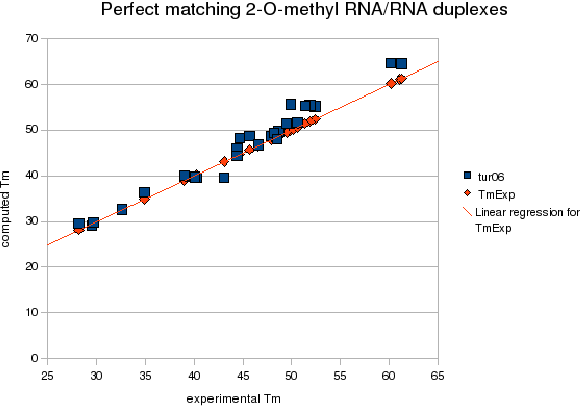
\includegraphics[width=1\linewidth]{images/DNAPerfectlyMatching}
\caption{Comparison of experimental and computed Tm for various sets of
  DNA nearest-neighbor parameters. $[\mbox{Na}^+] = 1$~M, $[\mbox{nucleic acid}] = 4\cdot{}10^{-4}$~M}
\end{figure}

\begin{figure}[h!]
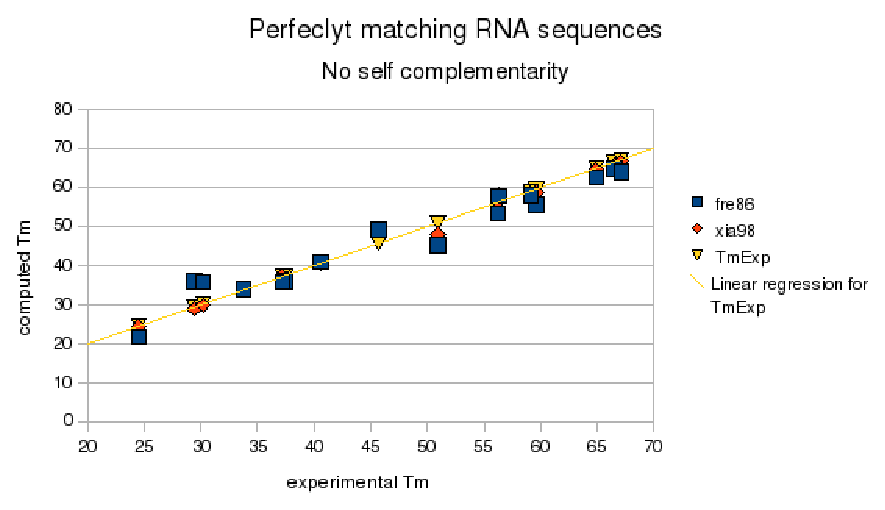
\includegraphics[width=1\linewidth]{images/RNAPerfectlyMatching}
\caption{Comparison of experimental and computed Tm for various sets of
  RNA nearest-neighbor parameters. $[\mbox{Na}^+] = 1$~M, $[\mbox{nucleic acid}] = 2\cdot{}10^{-4}$~M}
\end{figure}

\begin{figure}[h!]
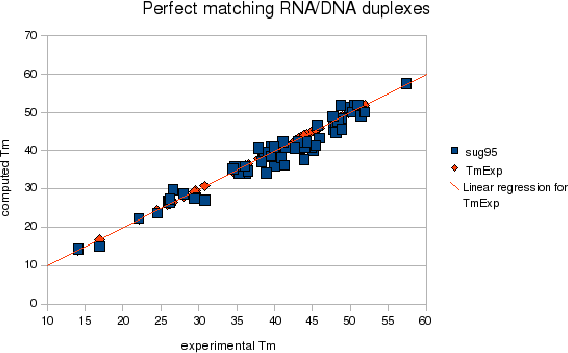
\includegraphics[width=1\linewidth]{images/DNARNA}
\caption{Comparison of experimental and computed Tm for various sets of
  DNA/RNA nearest-neighbor parameters. $[\mbox{Na}^+] = 1$~M, $[\mbox{nucleic acid}] = 1\cdot{}10^{-4}$~M}
\end{figure} 

\begin{figure}[h!]
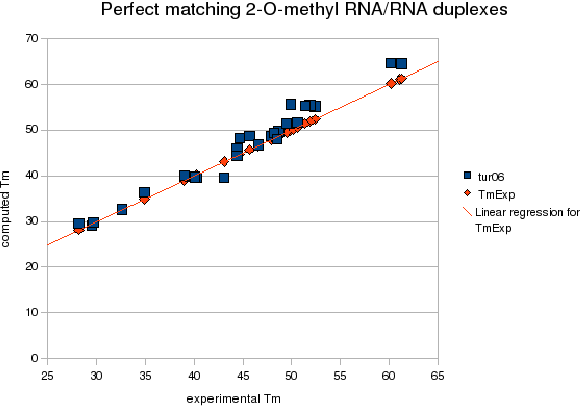
\includegraphics[width=1\linewidth]{images/mRNARNA}
\caption{Comparison of experimental and computed Tm for various sets of
  2-O-methyl RNA nearest-neighbor parameters. $[\mbox{Na}^+] = 1$~M, $[\mbox{nucleic acid}] = 1\cdot{}10^{-4}$~M}
\end{figure}

\pagebreak
\clearpage
\subsubsection{Sequences composed of CNG repeats}

If the sequence (sens 5'3') is a sequence of type \texttt{G(CNG)xC} where x is the number of CNG repeats in
the sequence and N a unique nucleic acid which will get bound to itself, we can use specific
experimental parameters to compute the enthalpy and entropy of the duplex formation. These parameters can be used
only for sequences composed from 2 to 7 CNG repeats and the initiation is already included.
 
\begin{displaymath}
  \begin{array}[t]{ccc}
  \Delta{}H&=&\Delta{}h_\mathrm{sequence-of-type-\texttt{G(CNG)xC}}\\
  \end{array}
\end{displaymath}
For further information, see the referenced article.

\begin{table}[hc]
\begin{tabular}[h]{| c | c | c |}
\textbf{model} & \textbf{limits} & \textbf{Article} \\
 \hline
\textbf{bro05} & RNA & Broda et al (2005) \\
 & Self complementary sequences & Biochemistry 44: 10873-10882\\
 & 2 to 7 CNG repeats & \\
 \hline
\end{tabular}
\end{table}


\textbf{Example} :
\begin{alltt}
G\textbf{CAGCAGCAG}C
C\textbf{GACGACGAC}G
\end{alltt}

\begin{multline*}
\Delta H {\mbox{\texttt{GCAGCAGCAGC}} \choose \mbox{\texttt{CGACGACGACG}}} = 
\Delta H {(\mbox{3-CAG-repeats})}
\end{multline*}

       (The same computation is performed for $\Delta S$)

\begin{figure}[h]
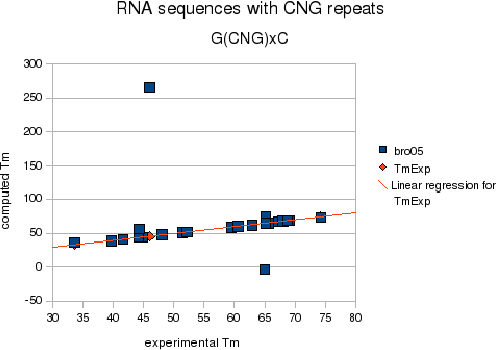
\includegraphics[width=1\linewidth]{images/CNG}
\caption{Comparison of experimental and computed Tm for various sets of
 RNA sequences composed of CNG repeats. $[\mbox{Na}^+] = 1$~M, $[\mbox{nucleic acid}] = 1\cdot{}10^{-4}$~M}
\end{figure}

\pagebreak
Be aware : The results for sequences composed of 4 or 5 CCG repeats is not reliable. (the figure shows two values
far from the expected temperature). This might be due to a majority of hairpin loop formation. See the article
above for further informations.

\subsubsection{Single mismatch effect}

The single mismatches are taken into account but the two first and positions cannot
be mismatched. in such a case, the result is unpredictable, and all cases are
possible. for instance (see Allawi and SanLucia 1997), the duplex
\begin{alltt}
A          T  
 \underline{G}TGAGCTCA\underline{T}  
 \underline{T}ACTCGAGT\underline{G}  
T          A   
\end{alltt}

is more stable than 

\begin{alltt}
A\underline{G}TGAGCTCA\underline{T}T 
T\underline{T}ACTCGAGT\underline{G}A 
\end{alltt}

For DNA duplexes, this program computes the hybridisation enthalpy and entropy from the elementary 
parameters of each Crick's pair containing the single mismatch. 
\begin{displaymath}
  \begin{array}[t]{ccc}
  \Delta{}h_\mathrm{single-mismatch}&=&\sum \delta{}h_\mathrm{Crick's-pair-containing-the-mismatch}\\
  \end{array}
\end{displaymath}

\textbf{Example} :
\begin{multline*}
\Delta H {\mbox{\texttt{ATC}} \choose \mbox{\texttt{TCG}}} = 
\Delta H {\mbox{\texttt{AT}} \choose \mbox{\texttt{TC}} } + 
\Delta H {\mbox{\texttt{TC}} \choose \mbox{\texttt{CG}} } \\
\end{multline*}

       (The same computation is performed for $\Delta S$)
       
\begin{figure}[h]
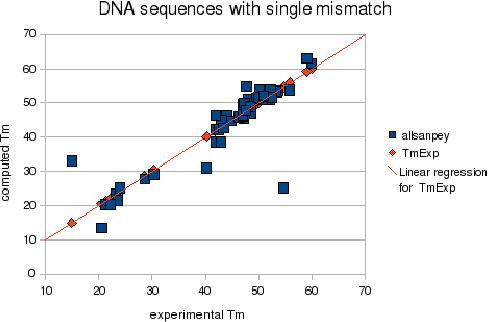
\includegraphics[width=1\linewidth]{images/DNASingleMismatch}
\caption{Comparison of experimental and computed Tm for various sets of
 DNA sequences containing one single mismatch. $[\mbox{Na}^+] = 1$~M, $[\mbox{nucleic acid}] = 4\cdot{}10^{-4}$~M}
\end{figure}

For RNA duplexes, the different models to computes the thermodynamic contribution of single mismatch to the helix coil 
stability are more complex.


\paragraph{\textbf{Model from Amber R. Davis and Brent M Znosco, 2007-2008}}

\begin{multline*}
\Delta h {(\mbox{single-mismatch})} = 
\delta{}h_\mathrm{mismatch-nucleotides} +
\delta{}h_\mathrm{mismatch-NN-interaction} +
\delta{}h_\mathrm{AU/GU} \\
\end{multline*}

Where :

$\delta{}h_\mathrm{mismatch-nucleotides}$ accounts for the identity of the single mismatch nucleotides.

$\delta{}h_\mathrm{mismatch-NN interaction}$ accounts for the interaction between the mismatch nucleotides and 
the nearest neighbors. (R purine, Y pyrimidine)

$\delta{}h_\mathrm{AU/GU}$ accounts for AU or GU nearest neighbors.

\textbf{Example} :
\begin{multline*}
\Delta H {\mbox{\texttt{AUC}} \choose \mbox{\texttt{UUG}}} = 
\Delta H {\mbox{\texttt{U}} \choose \mbox{\texttt{U}} } + 
1 \times \Delta H {\mbox{\texttt{AU}} } +
\Delta H {\mbox{\texttt{RYY}} \choose \mbox{\texttt{YYR}} } \\
\end{multline*}

       (The same computation is performed for $\Delta S$)
       

\paragraph{\textbf{Model from Zhi Johm Lu, Douglas H. Turner and David H. Mathews, 2006}}

\begin{multline*}
\Delta h {(\mbox{single-mismatch})} =
\delta{}h_\mathrm{initiation-loop-of-2} +
\delta{}h_\mathrm{per-AU/GU} +
\delta{}h_\mathrm{GG} +
\delta{}h_\mathrm{RU/YU}\\
\end{multline*}

Where :

$\delta{}h_\mathrm{initiation-loop-of-2}$ accounts for the initiation of a single non canonical pair.

$\delta{}h_\mathrm{GG}$ accounts for a GG single mismatch.

$\delta{}h_\mathrm{RU/YU}$ accounts for a 5'RU/3'YU stack with R a purine and Y a pyrimidine.

$\delta{}h_\mathrm{per-AU/GU}$ accounts for AU or GU nearest neighbors.

\textbf{Example} :
\begin{multline*}
\Delta H {\mbox{\texttt{AUC}} \choose \mbox{\texttt{UUG}}} =
\Delta H {\mbox{initiation-loop-of-2}} + 
1 \times \Delta H {\mbox{\texttt{per-AU}} } +
\Delta H {\mbox{\texttt{RU}} \choose \mbox{\texttt{YU}} } \\
\end{multline*}

       (The same computation is performed for $\Delta S$)
       
For further information, see the referenced articles.

\begin{table}[hc]
\begin{tabular}[h]{| c | c | c |}
\textbf{model} & \textbf{limits} & \textbf{Article} \\
 \hline
\textbf{allsanpey} & DNA & Allawi and SantaLucia (1997)\\
 & & Biochemistry 36: 10581-10594 \\
 & & Allawi and SantaLucia (1998)\\
 & & Biochemistry 37: 2170-2179 \\
 & & Allawi and SantaLucia (1998)\\
 & & Nuc Acids Res 26: 2694-2701 \\
 & & Allawi and SantaLucia (1998)\\
 & & Biochemistry 37: 9435-9444 \\
 & & Peyret et al. (1999)\\
 & & Biochemistry 38: 3468-3477 \\
 \hline 
tur06 & RNA & Douglas M Turner et al (2006)\\
 & & Nucleic Acids Research 34: 4912-4924 \\
 \hline
zno07 & RNA & Brent M Znosko et al (2007)\\
 & & Biochemistry 46: 13425-13436 \\
 \hline
\textbf{zno08} & RNA & Brent M Znosko et al (2008)\\
 & at least & Biochemistry 47: 10178-10187 \\
 & one adjacent & \\
 & GU base pair & \\
 \hline
\end{tabular}
\end{table}
\pagebreak

\begin{figure}[h]
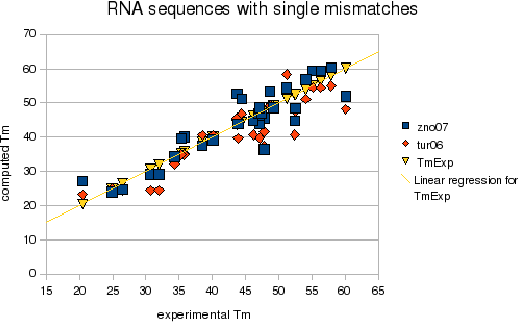
\includegraphics[width=1\linewidth]{images/RNASingleMismatch}
\caption{Comparison of experimental and computed Tm for various sets of
 RNA sequences containing one single mismatch. $[\mbox{Na}^+] = 1$~M, $[\mbox{nucleic acid}] = 1\cdot{}10^{-4}$~M}
\end{figure}

\clearpage
\subsubsection{Tandem mismatches effect}

The tandem mismatches (two adjacent mismatches) are taken into account but the two first and positions cannot
be mismatched. Moreover the thermodynamic parameters are still not available for every possible cases.
In such a case, the program, unable to compute any relevant result, will quit with a warning.

For DNA duplexes, this program computes the hybridisation enthalpy and entropy from the elementary 
parameters of each Crick's pair containing the mismatch(es). 
\begin{multline*}
\Delta{}h_\mathrm{tandem-mismatch} =
\delta{}h_\mathrm{Crick's-pair-containing-tandem-mismatch} \\ + 
\sum \delta{}h_\mathrm{Crick's-pair-containing-single-mismatch}
\end{multline*}


\textbf{Example} :
\begin{multline*}
\Delta H {\mbox{\texttt{ATGC}} \choose \mbox{\texttt{TCAG}}} = 
\Delta H {\mbox{\texttt{AT}} \choose \mbox{\texttt{TC}} } + 
\Delta H {\mbox{\texttt{TG}} \choose \mbox{\texttt{CA}} } + 
\Delta H {\mbox{\texttt{GC}} \choose \mbox{\texttt{AG}} } \\
\end{multline*}

       (The same computation is performed for $\Delta S$) 

\begin{figure}[h]
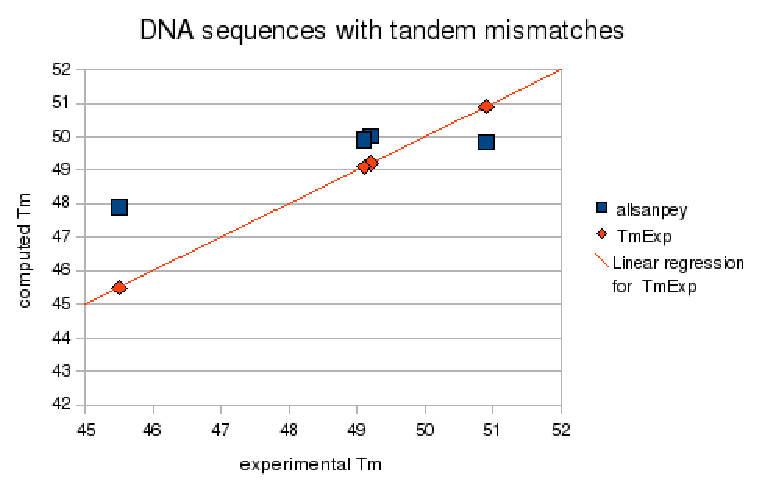
\includegraphics[width=1\linewidth]{images/DNATandemMismatch}
\caption{Comparison of experimental and computed Tm for various sets of
 DNA sequences containing one tandem mismatch. $[\mbox{Na}^+] = 1$~M, $[\mbox{nucleic acid}] = 4\cdot{}10^{-4}$~M}
\end{figure}

For RNA duplexes, the different models to computes the thermodynamic contribution of tandem mismatch to the helix coil 
stability are more complex.

\paragraph{Symmetric tandem mismatches : \textbf{Model from Zhi Johm Lu, Douglas H. Turner and David H. Mathews, 2006}}

\begin{multline*}
\Delta h {(\mbox{tandem-mismatch})} = 
\delta{}h_\mathrm{tandem-mismatch+closing-base-pairs} \\
\end{multline*}

Where :

$\delta{}h_\mathrm{mismatch-nucleotides}$ accounts for the identity of the double mismatch nucleotides and the identity of the base pairs
adjacent to the tandem mismatches.

\textbf{Example} :
\begin{multline*}
\Delta H {\mbox{\texttt{G AC C}} \choose \mbox{\texttt{C CA G}}} = 
\Delta H {\mbox{\texttt{AC}} \choose \mbox{\texttt{CA}}} -adjacent-to-GC\\
\end{multline*}

       (The same computation is performed for $\Delta S$)    

\paragraph{Asymmetric tandem mismatches : \textbf{Model from Zhi Johm Lu, Douglas H. Turner and David H. Mathews, 2006}}

\begin{multline*}
\Delta h {(\mbox{tandem-mismatch})} =
( \delta{}h_\mathrm{symmetric-duplex-1} +
\frac{\delta{}h_\mathrm{symmetric-duplex-2} )}{2} \\ +
\delta{}h_\mathrm{GG} +
\delta{}h_\mathrm{p}\\
\end{multline*}

Where :

$\delta{}h_\mathrm{symmetric-duplex-1}$ accounts for the enthalpy of a symmetric tandem mismatch composed of
the first closing base pair and the first mismatch nucleotides.

$\delta{}h_\mathrm{symmetric-duplex-2}$ accounts for the enthalpy of a symmetric tandem mismatch composed of
the second closing base pair and the second mismatch nucleotides.

$\delta{}h_\mathrm{GG}$ accounts for a GG pair adjacent to a AA pair or any non canonical pair containing a pyrimidine.

$\delta{}h_\mathrm{p}$ accounts for an AG or GA pairs adjacent to a UC, CC or CU pair and a UU pair adjacent to an AA pair .

\textbf{Example} :
\begin{multline*}
\Delta H {\mbox{\texttt{A GC C}} \choose \mbox{\texttt{U AU G}}} =
( \Delta H {\mbox{\texttt{A GA U}} \choose \mbox{\texttt{U AG A}}} + 
\Delta H {\mbox{\texttt{G UC C}} \choose \mbox{\texttt{C CU G}}} +
\Delta H {\mbox{\texttt{GA}} -adjacent-to- \mbox{\texttt{CU}} } \\
\end{multline*}

       (The same computation is performed for $\Delta S$)
       
For further information, see the referenced articles.

\begin{table}[hc]
\begin{tabular}[h]{| c | c | c |}
\textbf{model} & \textbf{limits} & \textbf{Article} \\
 \hline
\textbf{allsanpey} & DNA & Allawi and SantaLucia (1997) \\
 & only GT & Biochemistry 36: 10581-10594 \\
 & mismatches & Allawi and SantaLucia (1998) \\
 & and TA/TG & Biochemistry 37: 2170-2179 \\
 & mismatches & Allawi and SantaLucia (1998) \\
 & & Nuc Acids Res 26: 2694-2701 \\
 & & Allawi and SantaLucia (1998) \\
 & & Biochemistry 37: 9435-9444 \\
 & & Peyret et al. (1999) \\
 & & Biochemistry 38: 3468-3477\\
 \hline
\textbf{tur99} & RNA & Douglas M Turner et al (1999) \\
 & no adjacent & J.Mol.Biol.  288: 911-940 \\
 & GU or UG base & \\
 &  pairs & \\
 \hline
\end{tabular}
\end{table}

\begin{figure}[h]
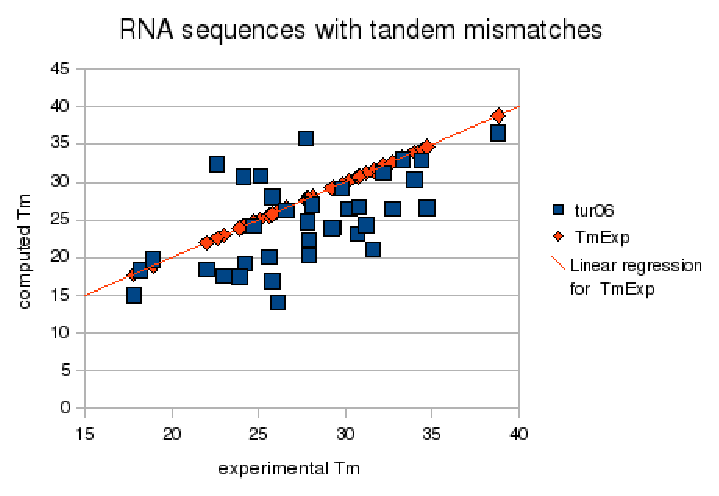
\includegraphics[width=1\linewidth]{images/RNATandemMismatch}
\caption{Comparison of experimental and computed Tm for various sets of
 RNA sequences containing one tandem mismatch. $[\mbox{Na}^+] = 1$~M, $[\mbox{nucleic acid}] = 1\cdot{}10^{-4}$~M}
\end{figure}

\clearpage
\subsubsection{Internal loop effect}

The internal loops (more than two adjacent mismatches) are taken into account but the two first and positions cannot
be mismatched. Moreover the thermodynamic parameters are still not available for every possible cases.
In such a case, the program, unable to compute any relevant result, will quit with a warning.
Moreover, the thermodynamics of the nucleic acids within the internal loop are salt 
independent and no salt correction will be applied to it. However, the thermodynamics
of the terminal mismatches are salt dependent and a salt correction will be applied
to them.
The thermodynamic model for DNA and RNA duplexes are similar.

\paragraph{DNA duplexes :\textbf{Model from John Santalucia, Jr. and Donald Hicks, 2004}} 

\begin{multline*}
\Delta h {(\mbox{internal-loop(n)})} =
\delta{}h_\mathrm{asymmetry} +
\delta{}h_\mathrm{left-terminal-mismatch} \\ +
\delta{}h_\mathrm{right-terminal-mismatch}\\
\Delta s {(\mbox{internal-loop(n)})} =
\delta{}s_\mathrm{loop(n)} +
\delta{}s_\mathrm{asymmetry} +
\delta{}s_\mathrm{left-terminal-mismatch} \\ +
\delta{}s_\mathrm{right-terminal-mismatch}\\
\end{multline*}

Where :

$\delta{}h_\mathrm{internal-loop(n)}$ accounts for the internal loop of n nucleotides.

$\delta{}h_\mathrm{asymmetry}$ accounts for the internal loop asymmetry (when the number of
nucleic acid within the internal loop is higher in one of the strand).

$\delta{}h_\mathrm{left-terminal-mismatch}$ accounts for the identity of the first mismatch 
nucleotides of the loop.

$\delta{}h_\mathrm{right-terminal-mismatch}$ accounts for the identity of the last mismatch 
nucleotides of the loop.

\textbf{Example} : Symmetric internal loop
\begin{multline*}
\Delta H {\mbox{\texttt{G ACCG C}} \choose \mbox{\texttt{C CATA G}}} = 
\Delta H {\mbox{\texttt{GA}} \choose \mbox{\texttt{CC}}} +
\Delta H {\mbox{\texttt{GC}} \choose \mbox{\texttt{AG}}}\\
\Delta S {\mbox{\texttt{G ACCG C}} \choose \mbox{\texttt{C CATA G}}} = 
\Delta S {\mbox{loop of 8}} +
\Delta S {\mbox{\texttt{GA}} \choose \mbox{\texttt{CC}}} +
\Delta S {\mbox{\texttt{GC}} \choose \mbox{\texttt{AG}}}\\
\end{multline*}

\paragraph{RNA duplexes :\textbf{Model from Zhi Johm Lu, Douglas H. Turner and David H. Mathews, 2006}}

\begin{multline*}
\Delta h {(\mbox{internal-loop(n)})} =
\delta{}h_\mathrm{initiation-loop(n)} +
\delta{}h_\mathrm{per-AU/GU} +
(n1 - n2) \delta{}h_\mathrm{asymmetry} \\ +
\delta{}h_\mathrm{first-non-canonical-pairs}\\
\end{multline*}


Where :

$\delta{}h_\mathrm{initiation-loop(n)}$ accounts for the internal loop of n nucleotides.

$\delta{}h_\mathrm{asymmetry}$ accounts for the internal loop asymmetry (when the number of
there is an unequal numbers of nucleotides on each side) with n1 and n2 the
number of nucleotides on each strand..

$\delta{}h_\mathrm{per_AU/GU}$ accounts for each AU or GU base pair adjacent
to the internal loop.

$\delta{}h_\mathrm{first-non-canonical-pairs}$ accounts for each sequence
specific first mismatch (bonus). It is not applied to loops of the form 1 \times (n-1) with
n > 2.


\textbf{Example} : asymmetric internal loop
\begin{multline*}
\Delta H {\mbox{\texttt{A ACCG C}} \choose \mbox{\texttt{U C-UA G}}} = 
\Delta H {\mbox{loop initiation(7)}} +
1 \times \Delta H {\mbox{\texttt{per-AU}}} +
(4 - 3)\Delta H {\mbox{asymmetry}}\\
\end{multline*}

       (The same computation is performed for $\Delta S$)    
       
For further information, see the referenced articles.

\begin{table}[hc]
\begin{tabular}[h]{| c | c | c |}
\textbf{model} & \textbf{limits} & \textbf{Article} \\
\hline
\textbf{san04} & DNA & Santalucia et al (2004) \\
 & missing asymmetry & Annu. Rev. Biophys. Biomol. Struct 33 : 415-440\\
 & penalty, & \\
 & not tested & \\
 & with experimental & \\
 & results & \\
 \hline
\textbf{tur06} & RNA & Douglas M Turner et al (2006) \\
 & not tested & Nucleic Acids Research 34: 4912-4924 \\
 & with experimental & \\
 & results & \\
 \hline
\end{tabular}
\end{table}

\begin{figure}[h]
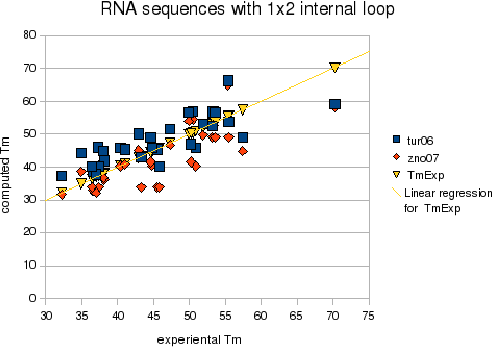
\includegraphics[width=1\linewidth]{images/1x2InternalLoop}
\caption{Comparison of experimental and computed Tm for various sets of
 RNA sequences containing one 1x2 internal loop. $[\mbox{Na}^+] = 1$~M, $[\mbox{nucleic acid}] = 1\cdot{}10^{-4}$~M}
\end{figure}

\pagebreak
\subsubsection{GU wobble base pairs effect}

The wobble GU base pairs are taken into account. This pairing is a non-Watson-Crick base pairing between two nucleotides 
in RNA molecules, but the thermodynamic stability of a wobble base pair is comparable to that of a Watson-Crick base pair.
Melting can also compute the thermodynamic of patterns with several adjacent GU base pairs.
This program computes the hybridisation enthalpy and entropy from the elementary 
parameters of each Crick's pair containing the GU base pairs.

\begin{displaymath}
  \begin{array}[t]{ccc}
  \Delta{}h_\mathrm{pattern-composed-of-GU-base-pairs}&=&\sum \delta{}h_\mathrm{Crick's pair-containing-GU-base-pairs}\\
  \end{array}
\end{displaymath}

\textbf{Examples} : One GU base pair
\begin{multline*}
\Delta H {\mbox{\texttt{GUC}} \choose \mbox{\texttt{CGG}}} = 
\Delta H {\mbox{\texttt{GU}} \choose \mbox{\texttt{CG}}} +
\Delta H {\mbox{\texttt{UC}} \choose \mbox{\texttt{GG}}}\\
\end{multline*}

\textbf{Examples} : Two adjacent GU base pairs
\begin{multline*}
\Delta H {\mbox{\texttt{GUGC}} \choose \mbox{\texttt{CGUG}}} = 
\Delta H {\mbox{\texttt{GU}} \choose \mbox{\texttt{CG}}} +
\Delta H {\mbox{\texttt{UG}} \choose \mbox{\texttt{GU}}} +
\Delta H {\mbox{\texttt{UC}} \choose \mbox{\texttt{GG}}}\\
\end{multline*}

       (The same computation is performed for $\Delta S$) 

       
For further information, see the referenced articles.

\begin{table}[hc]
\begin{tabular}[h]{| c | c | c |}
\hline
\textbf{model} & \textbf{limits} & \textbf{Article} \\
\textbf{tur99} & RNA & Douglas M Turner et al (1999) \\
 & & J.Mol.Biol.  288: 911-940 \\
\hline
\end{tabular}
\end{table}

\begin{figure}[h]
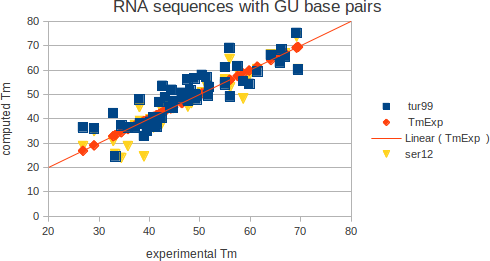
\includegraphics[width=1\linewidth]{images/GUBasePairs}
\caption{Comparison of experimental and computed Tm for various sets of
 RNA sequences containing GU base pairs. $[\mbox{Na}^+] = 1$~M, $[\mbox{nucleic acid}] = 1\cdot{}10^{-4}$~M}
\end{figure}

\subsubsection{Single dangling end effect}

The single dangling ends, that is the unmatched terminal nucleotides, can be taken into
account, but all the thermodynamic parameters are not available. In such a case, 
the result is unpredictable, and all cases are possible. 

For DNA and RNA duplexes, this program computes the hybridisation enthalpy and entropy from the elementary 
parameters of the Crick's pair containing the single dangling end. 
\begin{displaymath}
  \begin{array}[t]{ccc}
  \Delta{}h_\mathrm{single-dangling-end}&=&\delta{}h_\mathrm{Crick's-pair-containing-the-dangling-end}\\
  \end{array}
\end{displaymath}

\textbf{Example} :
If the duplex is :
\begin{alltt}
GCTAG\textbf{-}
CGATC\textbf{A}
\end{alltt}
\begin{multline*}
\Delta H {\mbox{\texttt{GCTAG-}} \choose \mbox{\texttt{CGATCCA}}} =
\Delta H {\mbox{perfectly-matching-sequence}} +
\Delta H {\mbox{single-dangling-end}} \\
\Delta H {\mbox{\texttt{GCTAG-}} \choose \mbox{\texttt{CGATCCA}}} =
\Delta H {\mbox{\texttt{GCTAG}} \choose \mbox{\texttt{CGATCC}}} +
\Delta H {\mbox{\texttt{G-}} \choose \mbox{\texttt{CA}}} \\
\end{multline*}


       (The same computation is performed for $\Delta S$)

For further information, see the referenced articles.

\begin{table}[hc]
\begin{tabular}[h]{| c | c | c |}
\textbf{model} & \textbf{limits} & \textbf{Article} \\
\hline
\textbf{bom00} & DNA & Bommarito et al. (2000) \\
 & & Nuc Acids Res 28: 1929-1934 \\
\hline
sugdna02 & DNA & Sugimoto et al. (2002) \\
 & only terminal & J. Am. Chem. Soc. 124: 10367-10372 \\
 & poly A & \\
 & self complementary & \\
 & sequences & \\
 \hline
sugrna02 & RNA & Sugimoto et al. (2002) \\
 & only terminal poly A & J. Am. Chem. Soc. 124: 10367-10372 \\
 & self complementary & \\
 & sequences & \\
 \hline
\textbf{ser08} & RNA & Martin J Serra et al. (2006) \\
 & only 3' UA, & Nucleic Acids research 34: 3338-3344 \\
 & GU and UG terminal & Martin J Serra et al. (2008) \\
 & base pairs & Nucleic Acids research 36: 5652-5659 \\
 & only 5' UG and GU & \\
 & terminal base pairs & \\
 \hline
\end{tabular}
\end{table}

\begin{figure}[h]
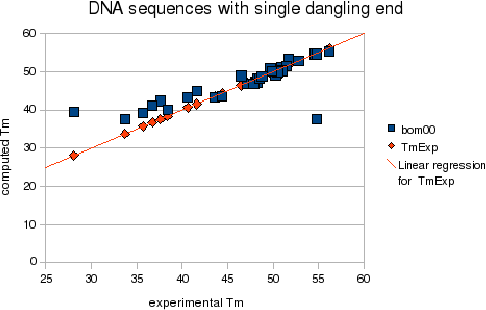
\includegraphics[width=1\linewidth]{images/DNASingleDanglingEnd}
\caption{Comparison of experimental and computed Tm for various sets of
 DNA sequences containing single dangling ends. $[\mbox{Na}^+] = 1$~M, $[\mbox{nucleic acid}] = 1\cdot{}10^{-4}$~M}
\end{figure}

\begin{figure}[h]
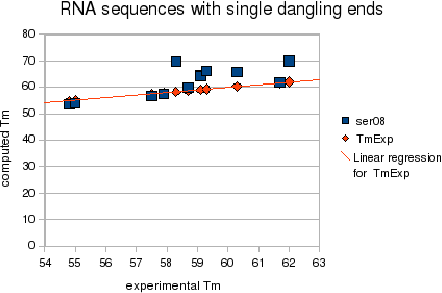
\includegraphics[width=1\linewidth]{images/RNASingleDanglingEnd}
\caption{Comparison of experimental and computed Tm for various sets of
 RNA sequences containing single dangling ends. $[\mbox{Na}^+] = 1$~M, $[\mbox{nucleic acid}] = 1\cdot{}10^{-4}$~M}
\end{figure}

\clearpage
\subsubsection{Double dangling end effect}

The double dangling ends, that is the two adjacent unmatched terminal nucleotides, can be taken into
account (mostly for RNA sequences). This program computes the hybridisation enthalpy and entropy in two times :
First, it computes the energy from the single dangling end as if the duplex contained
only a single danging end and then, it adds a bonus for the second dangling end if it is necessary. 
\begin{multline*}
\Delta{}h_\mathrm{double-dangling-end} =
\delta{}h_\mathrm{single-dangling-end} \\ + 
\delta{}h_\mathrm{bonus-second-dangling-end}\\
\end{multline*}

\textbf{Example} :

\begin{multline*}
\Delta H {\mbox{\texttt{UAC}} \choose \mbox{\texttt{A--}}} =
\Delta H {\mbox{UA}} +
\Delta H {\mbox{bonus-pyrimidine-purine-pyrimidine}} \\
\end{multline*}

       (The same computation is performed for $\Delta S$)

For further information, see the referenced articles.

\begin{table}[hc]
\begin{tabular}[h]{| c | c | c |}
\textbf{model} & \textbf{limits} & \textbf{Article} \\
\hline
sugdna02 & DNA & Sugimoto et al. (2002)\\
 & only terminal & J. Am. Chem. Soc. 124: 10367-10372 \\
 & poly A & \\
 & self complementary & \\
 & sequences & \\
 \hline
sugrna02 & RNA & Sugimoto et al. (2002)\\
 & only terminal & J. Am. Chem. Soc. 124: 10367-10372 \\
 & poly A & \\
 & self complementary & \\
 & sequences & \\
 \hline
ser05 & RNA & Martin J Serra et al. (2005)\\
 & depends on & RNA 11: 512-516 \\
 & the available & \\
 & thermodynamic & \\
 & parameters for & \\
 & single dangling & \\
 & ends & \\
 \hline
\textbf{ser06} & RNA & Martin J Serra et al. (2006)\\
 & & Nucleic Acids research 34: 3338-3344 \\
\hline
\end{tabular}
\end{table}

\begin{figure}[h]
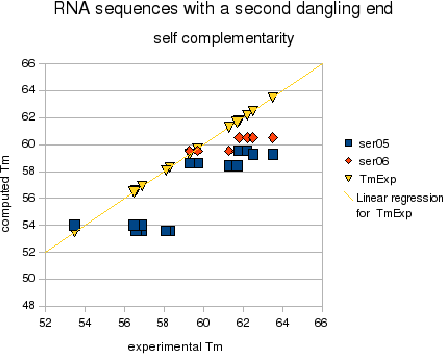
\includegraphics[width=1\linewidth]{images/RNASecondDanglingEnd}
\caption{Comparison of experimental and computed Tm for various sets of
 RNA sequences containing double dangling ends. $[\mbox{Na}^+] = 1$~M, $[\mbox{nucleic acid}] = 1\cdot{}10^{-4}$~M}
\end{figure}

\pagebreak
\subsubsection{Long dangling end effect (poly A)}

The long dangling ends, that is all the adjacent unmatched terminal nucleotides, can be taken into
account (only for polyA dangling ends for the moment). It is possible to compute the thermodynamic 
form one to four poly A dangling end. This program computes the hybridisation enthalpy 
and entropy from the parameters of the long dangling end with the adjacent terminal base pair.  
\begin{multline*}
\Delta{}h_\mathrm{long-dangling-end} =
\delta{}h_\mathrm{adjacent-terminal-base-pair+polyA} \\ 
\end{multline*}

\textbf{Example} :

If the duplex is :
\begin{alltt}
GCTAG\textbf{---}
CGATC\textbf{AAA}
\end{alltt}
\begin{multline*}
\Delta H {\mbox{\texttt{GCTAG---}} \choose \mbox{\texttt{CGATCCAAA}}} =
\Delta H {\mbox{perfectly-matching-sequence}} +
\Delta H {\mbox{long-dangling-end}} \\
\Delta H {\mbox{\texttt{GCTAG---}} \choose \mbox{\texttt{CGATCCAAA}}} =
\Delta H {\mbox{\texttt{GCTAG}} \choose \mbox{\texttt{CGATCC}}} +
\Delta H {\mbox{\texttt{G---}} \choose \mbox{\texttt{CAAA}}} \\
\end{multline*}

       (The same computation is performed for $\Delta S$)

For further information, see the referenced articles.

\begin{table}[hc]
\begin{tabular}[h]{| c | c | c |}
\textbf{model} & \textbf{limits} & \textbf{Article} \\
\hline
\textbf{sugdna02} & DNA & Sugimoto et al. (2002)\\
 & only terminal & J. Am. Chem. Soc. 124: 10367-10372 \\
 & poly A & \\
 & self complementary & \\
 & sequences & \\
 \hline
\textbf{sugrna02} & RNA & Sugimoto et al. (2002)\\
 & only terminal & J. Am. Chem. Soc. 124: 10367-10372 \\
 & poly A & \\
 & self complementary & \\
 & sequences & \\
 \hline
\end{tabular}
\end{table}

\begin{figure}[h]
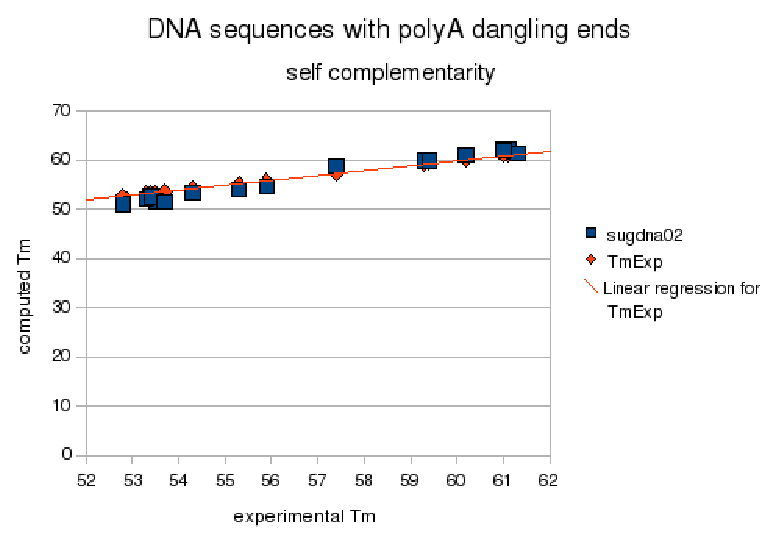
\includegraphics[width=1\linewidth]{images/DNALongDanglingEnd}
\caption{Comparison of experimental and computed Tm for various sets of DNA sequences containing long polyA dangling ends. $[\mbox{Na}^+] = 1$~M, $[\mbox{nucleic acid}] = 1\cdot{}10^{-4}$~M}
\end{figure}

\begin{figure}[h]
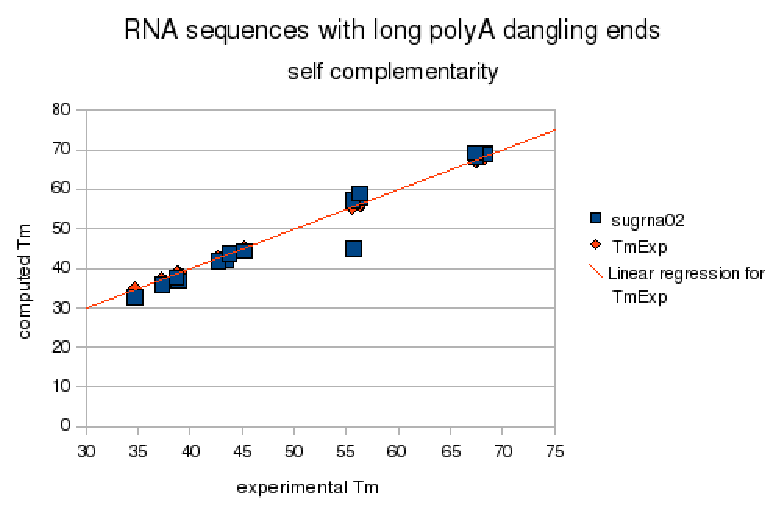
\includegraphics[width=1\linewidth]{images/RNALongDanglingEnd}
\caption{Comparison of experimental and computed Tm for various sets of RNA sequences containing long polyA dangling ends. $[\mbox{Na}^+] = 1$~M, $[\mbox{nucleic acid}] = 1\cdot{}10^{-4}$~M}
\end{figure}

\clearpage
\subsubsection{Single bulge loop effect}

The single bulge loops, that is the single unmatched internal nucleotides, can be taken into
account. , but all the thermodynamic parameters are not available. In such a case, 
the result is unpredictable, and all cases are possible. 
There are several different models to compute the thermodynamic of single bulge loop:

\paragraph{DNA and RNA duplexes :\textbf{nearest neighbor model "NNN"}} 

\begin{multline*}
\Delta h {(\mbox{single-bulge-loop})} =
\delta{}h_\mathrm{unpaired-nucleotid+adjacent-base-pairs} \\
\end{multline*}

\textbf{Example} :
If the duplex is :
\begin{alltt}
GCT\textbf{T}AGGC
CGA\textbf{-}TCCG
\end{alltt}
\begin{multline*}
\Delta H {\mbox{\texttt{GCTTAGGC}} \choose \mbox{\texttt{CGA-TCCG}}} =
\Delta H {\mbox{perfectly-matching-sequence-1}} +
\Delta H {\mbox{single-bulge-loop}} \\ +
\Delta H {\mbox{perfectly-matching-sequence-2}}\\
\Delta H {\mbox{\texttt{GCTTAGGC}} \choose \mbox{\texttt{CGA-TCCG}}} =
\Delta H {\mbox{\texttt{GCT}} \choose \mbox{\texttt{CGA}}} +
\Delta H {\mbox{\texttt{TTA}} \choose \mbox{\texttt{A-T}}} +
\Delta H {\mbox{\texttt{AGGC}} \choose \mbox{\texttt{TCCG}}}\\
\end{multline*}

       (The same computation is performed for $\Delta S$)   
  
 However, some types of single bulge loop can't be only modelled with a NNN nearest 
 neighbor model and the following models can give more reliable and accurate results (mostly
 for RNA single bulge loops.)  
  
\paragraph{DNA duplexes :\textbf{Model from John Santalucia, Jr. and Donald Hicks, 2004}} 

\begin{multline*}
\Delta h {(\mbox{single-bulge-loop})} =
\delta{}h_\mathrm{intervening-NN} +
\delta{}h_\mathrm{closing-AT-penalty}\\
\Delta s {(\mbox{single-bulge-loop})} =
\delta{}s_\mathrm{bulge-loop-of-1} +
\delta{}s_\mathrm{intervening-NN} +
\delta{}s_\mathrm{closing-AT-penalty}\\
\end{multline*}


Where :

$\delta{}h_\mathrm{bulge-loop-of-1}$ accounts for the bulge loop of 1 nucleotide.

$\delta{}h_\mathrm{intervening-NN}$ accounts for the intervening base pair stack.

$\delta{}h_\mathrm{closing-AT-penalty}$ accounts for each AT base pair adjacent
to the single bulge loop.

\textbf{Example} :

\begin{multline*}
\Delta H {\mbox{\texttt{GAC}} \choose \mbox{\texttt{C-G}}} =
\Delta H {\mbox{\texttt{GC}} \choose \mbox{\texttt{CG}}} \\
\Delta S {\mbox{\texttt{GAC}} \choose \mbox{\texttt{C-G}}} =
\Delta S {\mbox{bulge-loop-of-1}} +
\Delta S {\mbox{\texttt{GC}} \choose \mbox{\texttt{CG}}} \\
\end{multline*}

       (The same computation is performed for $\Delta S$) 

\paragraph{RNA duplexes :\textbf{Model from Zhi Johm Lu, Douglas H. Turner and David H. Mathews, 2006}} 

\begin{multline*}
\Delta h {(\mbox{single-bulge-loop})} =
\delta{}h_\mathrm{initiation-bulge-loop-of-1} +
\delta{}h_\mathrm{intervening-NN} \\
\end{multline*}


Where :

$\delta{}h_\mathrm{initiation-bulge-loop-of-1}$ accounts for the initiation of  bulge loop of 1 nucleotide.

$\delta{}h_\mathrm{intervening-NN}$ accounts for the intervening base pair stack.


\textbf{Example} :

\begin{multline*}
\Delta H {\mbox{\texttt{GAC}} \choose \mbox{\texttt{C-G}}} =
\Delta H {\mbox{initiation-bulge-loop-of-1}} +
\Delta H {\mbox{\texttt{GC}} \choose \mbox{\texttt{CG}}} \\
\end{multline*}

       (The same computation is performed for $\Delta S$) 
For further information, see the referenced articles.

\begin{table}[hc]
\begin{tabular}[h]{| c | c | c |}
\textbf{model} & \textbf{limits} & \textbf{Article} \\
\hline
\textbf{tan04} & DNA & Tanaka Fumiaki et al (2004)\\
 & & Biochemistry 43 : 7143-7150 \\
\hline
san04 & DNA & Santalucia et al (2004)\\
 & missing & Annu. Rev. Biophys. Biomol. Struct 33 : 415-440\\
 & closing AT & \\
 & penalty & \\
 \hline
ser07 & RNA & Martin J Serra et al (2007)\\
 & les reliable & Biochemistry 46 : 15123-15135 \\
 & results & \\
 & some missing & \\
 & parameters & \\
 \hline
\textbf{tur06} & RNA & Douglas M Turner et al (2006)\\
 & & Nucleic Acids Research 34: 4912-4924 \\
\hline
\end{tabular}
\end{table}

\begin{figure}[h]
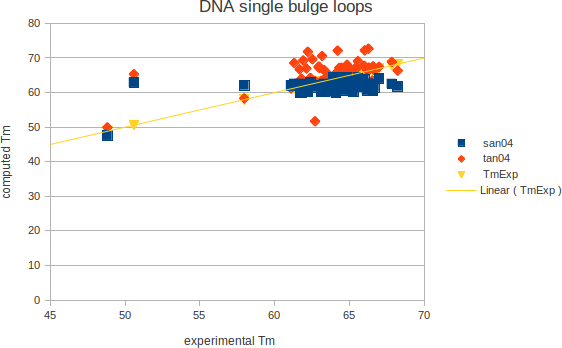
\includegraphics[width=1\linewidth]{images/DNASingleBulgeLoop}
\caption{Comparison of experimental and computed Tm for various sets of DNA sequences containing one single bulge loop. $[\mbox{Na}^+] = 1$~M, $[\mbox{nucleic acid}] = 1\cdot{}10^{-4}$~M}
\end{figure}

\begin{figure}[h]
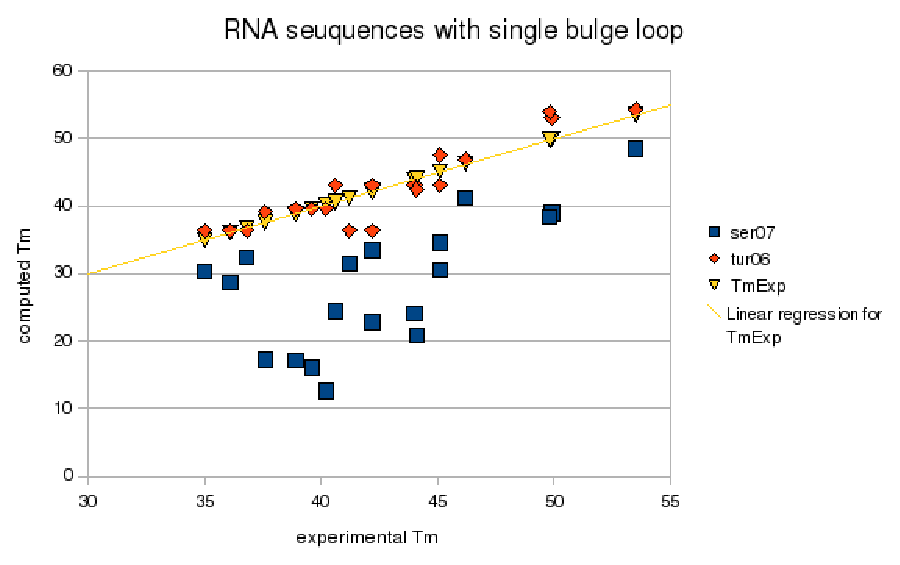
\includegraphics[width=1\linewidth]{images/RNASingleBulgeLoop}
\caption{Comparison of experimental and computed Tm for various sets of RNA sequences containing one single bulge loop. $[\mbox{Na}^+] = 1$~M, $[\mbox{nucleic acid}] = 1\cdot{}10^{-4}$~M}
\end{figure}

\clearpage
\subsubsection{long bulge loop effect}

The long bulge loops, that is all the adjacent unmatched internal nucleotides, can be taken into
account. , but all the thermodynamic parameters are not available. In such a case, 
the result is unpredictable, and all cases are possible. 
The RNA and DNA thermodynamic models are similar : 
  
\paragraph{DNA duplexes :\textbf{Model from John Santalucia, Jr. and Donald Hicks, 2004}} 

\begin{multline*}
\Delta h {(\mbox{long-bulge-loop})} =
\delta{}h_\mathrm{closing-AT-penalty}\\
\Delta s {(\mbox{single-bulge-loop})} =
\delta{}s_\mathrm{bulge-loop-of-n} +
\delta{}s_\mathrm{closing-AT-penalty}\\
\end{multline*}


Where :

$\delta{}h_\mathrm{bulge-loop-of-n}$ accounts for the bulge loop of n nucleotides.

$\delta{}h_\mathrm{closing-AT-penalty}$ accounts for each AT base pair adjacent
to the long bulge loop.

\textbf{Example} :

\begin{multline*}
\Delta H {\mbox{\texttt{GACGC}} \choose \mbox{\texttt{C---G}}} =
0
\Delta S {\mbox{\texttt{GACGC}} \choose \mbox{\texttt{C---G}}} =
\Delta S {\mbox{bulge-loop-of-3}} \\
\end{multline*}

\paragraph{RNA duplexes : \textbf{Model from Zhi Johm Lu, Douglas H. Turner and David H. Mathews, 2006}} 

\begin{multline*}
\Delta h {(\mbox{long-bulge-loop})} =
\delta{}h_\mathrm{initiation-bulge-loop-of-n} \\ +
\delta{}h_\mathrm{per-AU/GU-penalty}\\
\end{multline*}


Where :

$\delta{}h_\mathrm{initiation-bulge-loop-of-n}$ accounts for the initiation of the bulge loop of n nucleotides.

$\delta{}h_\mathrm{per-AU/GU-penalty}$ accounts for each AU or GU base pair adjacent
to the long bulge loop.


\textbf{Example} :

\begin{multline*}
\Delta H {\mbox{\texttt{AACGC}} \choose \mbox{\texttt{U---G}}} =
\Delta H {\mbox{initiation-bulge-loop-of-3}} +
1 \times \Delta H {\mbox{per-AU-penalty}} \\
\end{multline*}

       (The same computation is performed for $\Delta S$) 

For further information, see the referenced articles.

\begin{table}[hc]
\begin{tabular}[h]{| c | c | c |}
\textbf{model} & \textbf{limits} & \textbf{Article} \\
\hline
\textbf{san04} & DNA & Santalucia et al (2004)\\
 & missing closing & Annu. Rev. Biophys. Biomol. Struct 33 : 415-440\\
 & AT penalty & \\
 & not tested & \\
 & with experimental & \\
 & results & \\
 \hline
\textbf{tur06} & RNA & Douglas M Turner et al (2006)\\
 & not tested & Nucleic Acids Research 34: 4912-4924 \\
 & with experimental & \\
 & results & \\
 \hline
\end{tabular}
\end{table}

\subsubsection{Inosine bases effect}

The inosine bases (I) are taken into account, but all the thermodynamic parameters are not available. 
In such a case, the result is unpredictable, and all cases are possible, so the
program quit with a warning. For the RNA duplexes, only the thermodynamic parameters
for IU base pairs are available for the moment.
This program computes the hybridisation enthalpy and entropy from the elementary 
parameters of each Crick's pair containing the inosine base.

\begin{displaymath}
  \begin{array}[t]{ccc}
  \Delta{}h_\mathrm{pattern-containing-inosine-bases}&=&\sum
  \delta{}h_\mathrm{Crick's pair-containing-inosine-bases}\\
  \end{array}
\end{displaymath}

\textbf{Examples} : One inosine base
\begin{multline*}
\Delta H {\mbox{\texttt{AIC}} \choose \mbox{\texttt{TAG}}} = 
\Delta H {\mbox{\texttt{AI}} \choose \mbox{\texttt{TA}}} +
\Delta H {\mbox{\texttt{IC}} \choose \mbox{\texttt{AG}}}\\
\end{multline*}

\textbf{Examples} : Two adjacent base pairs containing inosine
\begin{multline*}
\Delta H {\mbox{\texttt{GIAC}} \choose \mbox{\texttt{CAIG}}} = 
\Delta H {\mbox{\texttt{GI}} \choose \mbox{\texttt{CA}}} +
\Delta H {\mbox{\texttt{IA}} \choose \mbox{\texttt{AI}}} +
\Delta H {\mbox{\texttt{AC}} \choose \mbox{\texttt{IG}}}\\
\end{multline*}

       (The same computation is performed for $\Delta S$) 
       
For further information, see the referenced articles.

\begin{table}[hc]
\begin{tabular}[h]{| c | c | c |}
\textbf{model} & \textbf{limits} & \textbf{Article} \\
\hline
\textbf{san05} & DNA & Santalucia et al.(2005)\\
 & missing parameters & Nucleic acids research 33 : 6258-6267 \\
 & for tandem & \\
 & base pairs & \\
 & containing & \\
 & inosine bases & \\
 \hline
\textbf{zno07} & RNA & Brent M Znosko et al. (2005)\\
 & only IU base & Biochemistry 46 : 4625-4634 \\
 & pairs & \\
 \hline
\end{tabular}
\end{table}

\begin{figure}[h]
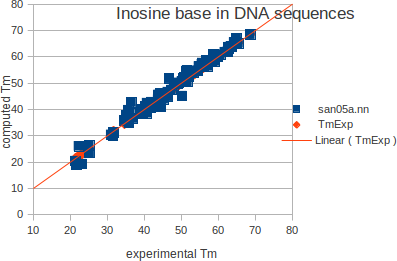
\includegraphics[width=1\linewidth]{images/DNAInosine}
\caption{Comparison of experimental and computed Tm for various sets of
 DNA sequences containing inosine. $[\mbox{Na}^+] = 1$~M, $[\mbox{nucleic acid}] = 1\cdot{}10^{-4}$~M}
\end{figure}

\begin{figure}[h]
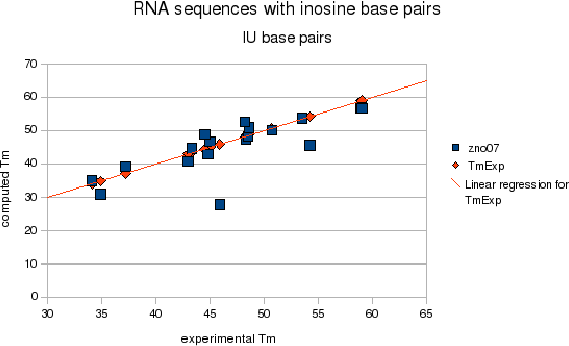
\includegraphics[width=1\linewidth]{images/RNAInosine}
\caption{Comparison of experimental and computed Tm for various sets of
 RNA sequences containing inosine. $[\mbox{Na}^+] = 1$~M, $[\mbox{nucleic acid}] = 1\cdot{}10^{-4}$~M}
\end{figure}

\clearpage
\subsubsection{Azobenzenes effect}

The trans azobenzenes (X\_T) and cis azobenzenes (X\_C) in DNA duplexes are taken 
into account. Be aware : when the number of cis azobenzenes increases in the sequence, 
the predictions are less accurate and less reliable.

\begin{multline*}
  \Delta{}h_\mathrm{pattern-containing-azobenzene} =
  \delta{}h_\mathrm{Crick's pair-containing-azobenzene+adjacent-base-pairs}\\
\end{multline*}

\textbf{Example} :
If the duplex is :
\begin{alltt}
GCT\textbf{X\_C}AGGC
CGATCCG
\end{alltt}
\begin{multline*}
\Delta H {\mbox{\texttt{GCTX\_CAGGC}} \choose \mbox{\texttt{CGATCCG}}} =
\Delta H {\mbox{perfectly-matching-sequence-1}} +
\Delta H {\mbox{azobenzene}} \\ +
\Delta H {\mbox{perfectly-matching-sequence-2}}\\
\Delta H {\mbox{\texttt{GCTX\_CAGGC}} \choose \mbox{\texttt{CGATCCG}}} =
\Delta H {\mbox{\texttt{GCT}} \choose \mbox{\texttt{CGA}}} +
\Delta H {\mbox{\texttt{TX\_CA}} \choose \mbox{\texttt{AT}}} +
\Delta H {\mbox{\texttt{AGGC}} \choose \mbox{\texttt{TCCG}}}\\
\end{multline*}

       (The same computation is performed for $\Delta S$) 
       
For further information, see the referenced articles.

\begin{table}[hc]
\begin{tabular}[h]{| c | c | c |}
\textbf{model} & \textbf{limits} & \textbf{Article} \\
\hline
\textbf{asa05} & DNA & Asanuma et al. (2005) \\
 & less reliable & Nucleic acids Symposium Series 49 : 35-36 \\
 & results when & \\
 & the number & \\
 & of cis azobenzene & \\
 & increases & \\
 \hline
\end{tabular}
\end{table}

\begin{figure}[h]
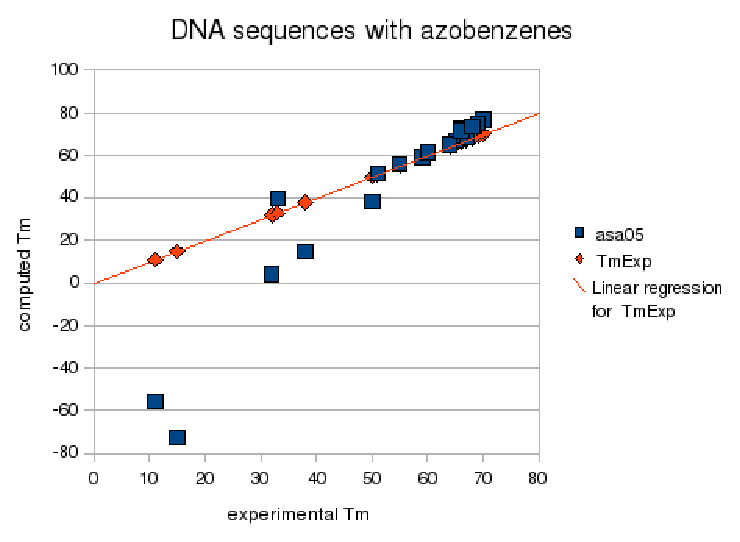
\includegraphics[width=1\linewidth]{images/Azobenzene}
\caption{Comparison of experimental and computed Tm for various sets of
 DNA sequences containing azobenzene. $[\mbox{Na}^+] = 1$~M, $[\mbox{nucleic acid}] = 2\cdot{}10^{-6}$~M}
\end{figure}

\pagebreak
\subsubsection{2-Hydroxyadenine bases effect}

The 2-hydroxyadenine bases (A*) in DNA duplexes are taken into account, but only in this two different
sequence contexts : 5' GA*C 3' and 5' TA*A 3'. The program computes the enthalpy and the entropy in two
times : first it computes the enthalpy and entropy of the two Crick's pairs containing the hydroxyadenine
as if the base pair containing the hydroxyadenine was a simple AT base pair, and then it computes the hydroxyadenine
increments.

\begin{multline*}
\Delta{}h_\mathrm{pattern-containing-hydroxyadenine} =
\sum \delta{}h_\mathrm{Crick's pair-with-AT-base-pair} \\ +
\delta{}h_\mathrm{hydroxyadenine-increment}
\end{multline*}

\textbf{Examples}
\begin{multline*}
\Delta H {\mbox{\texttt{GA*C}} \choose \mbox{\texttt{CCG}}} = 
\Delta H {\mbox{\texttt{GA}} \choose \mbox{\texttt{CT}}} +
\Delta H {\mbox{\texttt{AC}} \choose \mbox{\texttt{CG}}} \\ +
\Delta H {\mbox{increment-for-GA*C/CCG}}\\
\end{multline*}

       (The same computation is performed for $\Delta S$) 
       
For further information, see the referenced articles.

\begin{table}[hc]
\begin{tabular}[h]{| c | c | c |}
\textbf{model} & \textbf{limits} & \textbf{Article} \\
\hline
\textbf{sug01} & DNA & Sugimoto et al.(2001)\\
 & only in 5' & Nucleic acids research 29 : 3289-3296\\
 & GA*C 3' & \\
 & and 5' TA*A & \\
 & contexts & \\
 \hline
\end{tabular}
\end{table}

\begin{figure}[h]
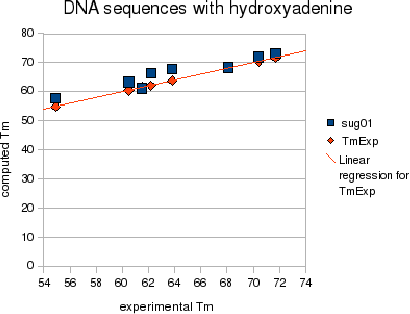
\includegraphics[width=1\linewidth]{images/Hydroxyadenine}
\caption{Comparison of experimental and computed Tm for various sets of
 DNA sequences containing hydroxyadenine. $[\mbox{Na}^+] = 1$~M, $[\mbox{nucleic acid}] = 1\cdot{}10^{-4}$~M}
\end{figure}

\subsubsection{Locked nucleic acids effect}

The locked nucleic acids (AL, GL, CL, TL) in DNA duplexes are taken into account.
The program computes the enthalpy and the entropy in two times : first it computes the enthalpy and entropy of 
the two Crick's pairs containing the locked nucleic acid as if the locked nucleic acid was a simple nucleic acid,
and then it computes the locked nucleic acid increments for each Crick's base pair containing the locked nucleic acid.

\begin{multline*}
\Delta{}h_\mathrm{pattern-containing-Locked-Nucleic-Acid} =
\sum \delta{}h_\mathrm{Crick's pair-without-Locked-Nucleic-Acid} \\ +
\sum \delta{}h_\mathrm{increment-Crick's pair-with-Locked-Nucleic-Acid}
\end{multline*}

\textbf{Examples}
\begin{multline*}
\Delta H {\mbox{\texttt{GALC}} \choose \mbox{\texttt{CTG}}} = 
\Delta H {\mbox{\texttt{GA}} \choose \mbox{\texttt{CT}}} +
\Delta H {\mbox{\texttt{AC}} \choose \mbox{\texttt{CG}}} \\ +
\Delta H {\mbox{increment-for-GAL/CT}} +
\Delta H {\mbox{increment-for-ALC/TG}}\\
\end{multline*}

       (The same computation is performed for $\Delta S$) 
       
For further information, see the referenced articles.

\begin{table}[hc]
\begin{tabular}[h]{| c | c | c |}
\textbf{model} & \textbf{limits} & \textbf{Article} \\
\hline
\textbf{mct04} & DNA & McTigue et al.(2004)\\
 & & Biochemistry 43 : 5388-5405\\
\hline
\end{tabular}
\end{table}

\begin{figure}[h]
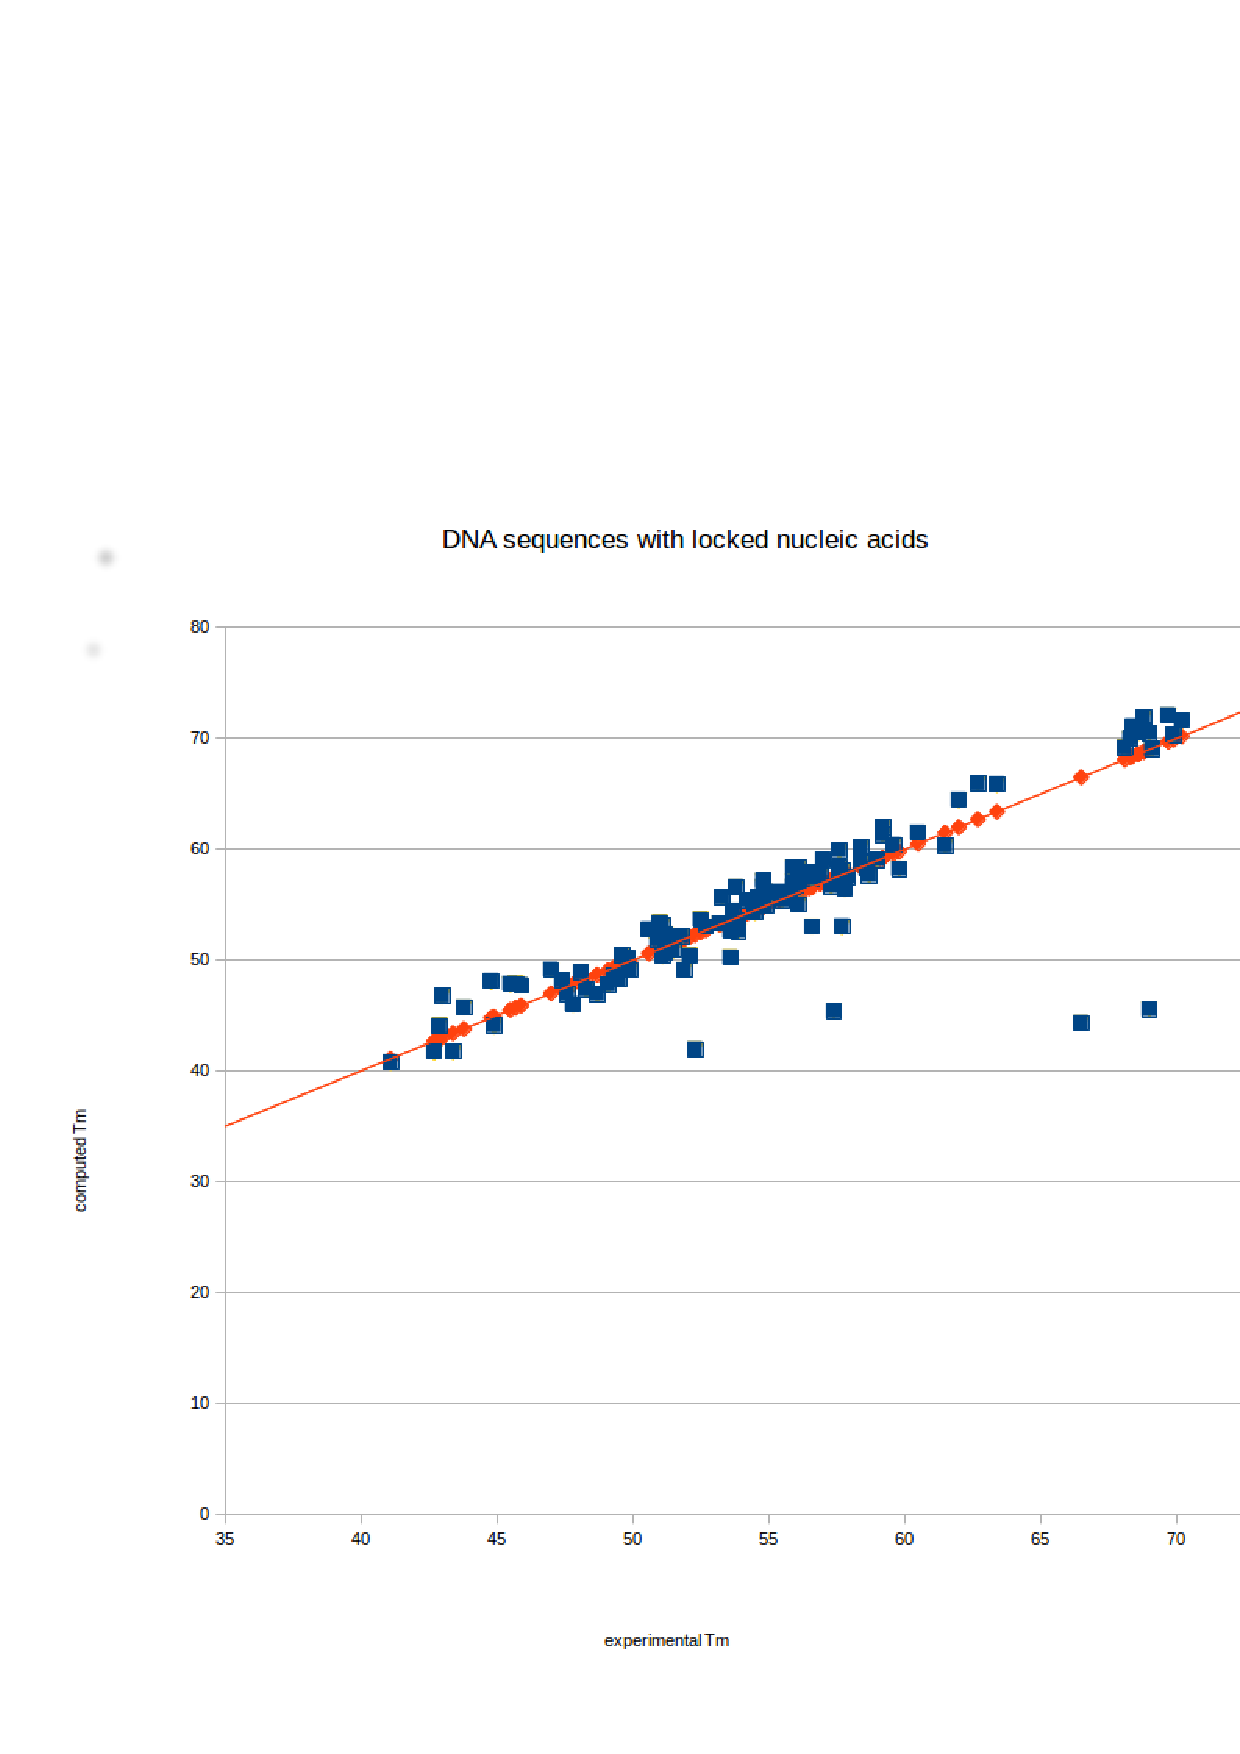
\includegraphics[width=1\linewidth]{images/LockedNucleicAcid}
\caption{Comparison of experimental and computed Tm for various sets of
 DNA sequences containing Locked Nucleic Acids. $[\mbox{Na}^+] = 1$~M, $[\mbox{nucleic acid}] = 5\cdot{}10^{-6}$~M}
\end{figure}
      
\subsection{The melting temperature }  

Then the melting temperature is computed by the following formula: 
 
 

\begin{tabular}[h]{rcp{1.6in}p{2.2in}}
Tm & = & \begin{math} \frac{\Delta{}H}{\Delta{}S + R \ln (C_T/F)} - 273.15 \end{math} \\
   &   &                                                                                                                                                \\
   &   & \footnotesize \textit{Tm} in K (for [Na$^+$] = 1~M)
\end{tabular}



In case of self complementary sequences, if the sequence (5' 3') is a sequence of type G(CNG)xC 
and x > 4, the sequence mainly turns into hairpin loops and this program will compute the melting
temperature with this formula :


   
\begin{tabular}[h]{rcp{1.6in}p{2.2in}}
Tm & = & \begin{math} \frac{\Delta{}H}{\Delta{}S} - 273.15 \end{math} \\
   &   &                                                                                                                                                \\
   &   & \footnotesize \textit{Tm} in K 
\end{tabular}


Moreover, no ion correction will be applied to this formula.

\subsection{Correction for the concentration of nucleic acid }  

\textit{F} is 1 in the case of self-complementarity oligonucleotides. If the
ODNs are not self-complementary, \textit{F} is 4 if both strands are present in
equivalent amount and \textit{F} is 2 if one strand is in excess (for instance
in \textsc{pcr} experiments).  Actually in the latter case, the formula would
have to use the difference of concentrations rather than the total
concentration. But if the excess is sufficient, the total concentration can be
assumed to be identical to the concentration of the strand in excess. That is,
if one strand is in excess, the actual formula is effectively $(C_{\mbox{max}} -
C_{\mbox{min}})/2$ but if $C_{\mbox{max}} \gg C_{\mbox{min}}$, $C_{\mbox{max}}
- C_{\mbox{min}}$ is close to the total concentration $C_T$.  If $C_{\mbox{max}}$ is close
to $C_{\mbox{min}}$, $(C_{\mbox{max}} - C_{\mbox{min}})/2$ is equivalent to $C_T/4$, which is the default
correction.

\textit{F} is 4 by default but note that \textsc{melting} can detect self complementary sequences 
for perfectly matching sequences even though there is(are) dangling end(s). In this case, the program will 
automatically change \textit{F} to 1. In addition to that, the computation takes an entropic term to correct 
for self-complementarity.
In case of other self complementary sequences which doesn't match perfetcly, the option \textit{-self} must be
used to inform the program of the self complementarity.

\begin{figure}[h]
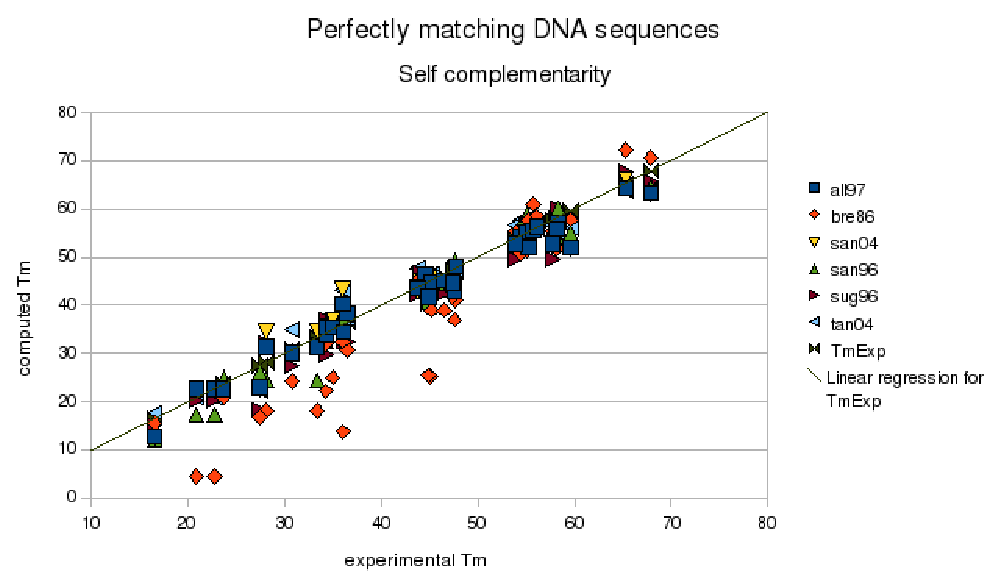
\includegraphics[width=1\linewidth]{images/DNASelfComplementarity}
\caption{Comparison of experimental and computed Tm for various sets of
 DNA self complementary sequences. $[\mbox{Na}^+] = 1$~M, $[\mbox{nucleic acid}] = 1\cdot{}10^{-4}$~M}
\end{figure} 

\begin{figure}[h]
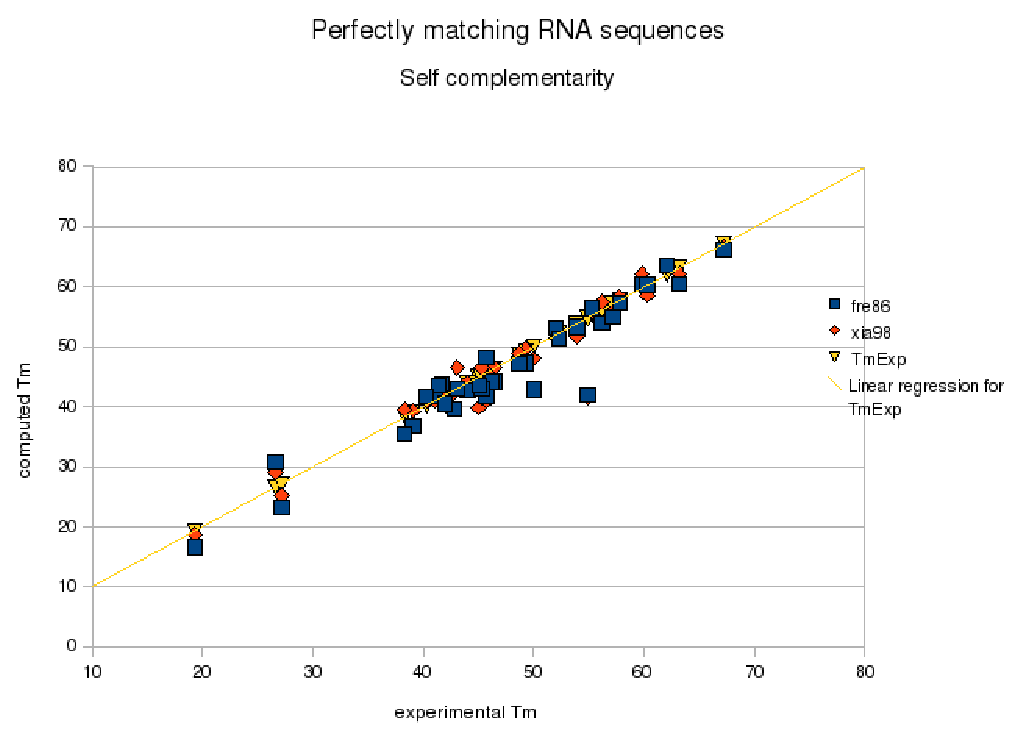
\includegraphics[width=1\linewidth]{images/RNASelfComplementarity}
\caption{Comparison of experimental and computed Tm for various sets of
 RNA self complementary sequences. $[\mbox{Na}^+] = 1$~M, $[\mbox{nucleic acid}] = 1\cdot{}10^{-4}$~M}
\end{figure}     
  
\clearpage
\subsection{Correction for the concentration of cations}  

After the program computed the melting temperature for $[\mbox{Na}^+]$=1, an ion correction wille be applied
either directly on the computed melting temperature or on the computed entropy. In the last case, the melting
temperature is computed using the first formula of the \textit{Melting temperature} section.
We must enter at least one of the following ion concentrations : $[\mbox{Na}^+]$, $[\mbox{K}^+]$, $[\mbox{Tris}^+]$ or
$[\mbox{Mg}^{2+}]$ and several ion corrections are proposed  (see the reference table to have more information):

\subsubsection{Sodium corrections}
 \begin{itemize}
 \item \textit{ahs01}
 \begin{displaymath}
  \Delta{}S=\Delta{}S_{[\mbox{Na}^+]=1\;\mathrm{M}}+0.847 \times (N - 1) \times \log [\mbox{Na}^+]   
 \end{displaymath}
 Where \emph{N} is the length of the duplex.
 \item \textit{kam71}
 \begin{displaymath}
  Tm=Tm_{[\mbox{Na}^+]=1\;\mathrm{M}}+(7.95 - 3.06 \times \Chi_{GC}) \times \ln [\mbox{Na}^+]  
 \end{displaymath}
 Where \emph{$\Chi_{GC}$} is the frequence of GC base pairs in the duplex.
 \item \textit{marschdot}
 \begin{displaymath}
  Tm=Tm_{[\mbox{Na}^+]=1\;\mathrm{M}}+ (8.75 - 2.83 \times \Chi_{GC}) \times \ln [\mbox{Na}^+]  
 \end{displaymath}
 Where \emph{$\Chi_{GC}$} is the frequence of GC base pairs in the duplex.
 \item \textit{owc1904}
 \begin{displaymath}
  Tm=Tm_{[\mbox{Na}^+]=1\;\mathrm{M}}+ (-3.22 \times \Chi_{GC} - 6.39) \times \ln [\mbox{Na}^+]  
 \end{displaymath}
 Where \emph{$\Chi_{GC}$} is the frequence of GC base pairs in the duplex.
 \item \textit{owc2004}
 \begin{displaymath}
 \frac{1}{Tm}=\frac{1}{Tm_{[\mbox{Na}^+]=1\;\mathrm{M}}}+ (3.85 \times \Chi_{GC} - 6.18) \times \frac{1}{100000} \times \ln [\mbox{Na}^+]  
 \end{displaymath}
 Where \emph{$\Chi_{GC}$} is the frequence of GC base pairs in the duplex.
 \item \textit{owc2104}
 \begin{displaymath}
 Tm=Tm_{[\mbox{Na}^+]=1\;\mathrm{M}}+ (-4.62 \times \Chi_{GC} + 4.52) \times \ln [\mbox{Na}^+] 
 \end{displaymath}
 \begin{displaymath}
 - 0.985 \times \ln [(\mbox{Na}^+)^2]  
 \end{displaymath}
 Where \emph{$\Chi_{GC}$} is the frequence of GC base pairs in the duplex.
 \item \textit{owc2204}
 \begin{multline*}
 \frac{1}{Tm}=\frac{1}{Tm_{[\mbox{Na}^+]=1\;\mathrm{M}}}+ (4.29 \times \Chi_{GC} - 3.95) \times 
 \end{multline*}
 \begin{multline*}
 \frac{1}{100000} \times \ln [\mbox{Na}^+] +
 9.40 \times \frac{1}{1000000} \times \ln [\mbox{Na}^+]
 \end{multline*}
 Where \emph{$\Chi_{GC}$} is the frequence of GC base pairs in the duplex.
 \item \textit{san96}
 \begin{displaymath}
  12.5  \log [\mbox{Na}^+]   
 \end{displaymath}
 \item \textit{san04}
 \begin{displaymath}
  \Delta{}S=\Delta{}S_{[\mbox{Na}^+]=1\;\mathrm{M}}+ 0.368 * (N - 1) \times \ln [\mbox{Na}^+]   
 \end{displaymath}
 Where \emph{N} is the length of the duplex.
 \item \textit{schlif}
 \begin{displaymath}
  Tm=Tm_{[\mbox{Na}^+]=1\;\mathrm{M}}+ 16.6 \times \log [\mbox{Na}^+]   
 \end{displaymath}
 \item \textit{tanna06}
 \begin{displaymath}
  \Delta{}S=\Delta{}S_{[\mbox{Na}^+]=1\;\mathrm{M}}- 3.22 \times (N - 1) \times g1  
 \end{displaymath}
 Where \emph{N} is the length of the duplex.
 \begin{displaymath}
  g1=a1 + \frac{b1}{N}  
 \end{displaymath}
 \begin{displaymath}
  a1= -0.07 \times \ln [\mbox{Na}^+] + 0.012 \times (\ln [\mbox{Mg}^{2+}])^2  
 \end{displaymath}
 \begin{displaymath}
  b1= 0.013 \times (\ln [\mbox{Mg}^{2+}])^2  
 \end{displaymath}
 item \textit{tanna07}
 \begin{displaymath}
  \Delta{}S=\Delta{}S_{[\mbox{Na}^+]=1\;\mathrm{M}}- 3.22 \times (N - 1) \times g1  
 \end{displaymath}
 Where \emph{N} is the length of the duplex.
 \begin{displaymath}
  g1=a1 + \frac{b1}{N}  
 \end{displaymath}
 \begin{displaymath}
  a1= -0.075 \times \ln [\mbox{Na}^+] + 0.012 \times (\ln [\mbox{Mg}^{2+}])^2  
 \end{displaymath}
 \begin{displaymath}
  b1= 0.018 \times (\ln [\mbox{Mg}^{2+}])^2  
 \end{displaymath}
 \item \textit{wet91}
 \begin{displaymath}
  Tm=Tm_{[\mbox{Na}^+]=1\;\mathrm{M}}+ 16.6  \log \frac{[\mbox{Na}^+]}{1 + 0.7 [\mbox{Na}^+]} + 3.85    
 \end{displaymath}
 \end{itemize}
 
\begin{table}[hc]
\begin{tabular}[h]{| c | c | c |}
\textbf{correction} & \textbf{contexts} & \textbf{Article} \\
\hline
ahs01 & DNA & Nicolas Von Ahsen et al ,2001 \\
 & Na>0 & Clinical Chemistry, 47, 1956-1961.\\
 \hline
kam71 & DNA & Frank-Kamenetskii et al. 1971 \\
 & Na>=0.069  & Biopolymers 10, 2623-2624.\\
 & Na<=1.02  & \\
 \hline
marschdot & DNA & Marmur, J., and Doty, P. (1962) \\
 & Na>=0.069  & J. Mol. Biol. 5, 109-118.\\
 & Na<=1.02 & Blake and Delcourt. (1998) Nucleic Acids Res. 26, 3323-3332 \\ 
 & & and corrigendum.\\
 \hline
owc1904 & DNA & Richard Owczarzy et al.,2004  \\
 & Na>0 & Biochemistry,43, 3537-3554.\\
 \hline
owc2004 & DNA & Richard Owczarzy et al., 2004 \\
 & Na>0 & Biochemistry, 43, 3537-3554.\\ 
 \hline
owc2104 & DNA & Richard Owczarzy et al., 2004 \\
 & Na>0 & Biochemistry, 43, 3537-3554.\\
 \hline 
\textbf{owc2204} & DNA & Richard Owczarzy et al., 2004 \\
 & Na>0 & Biochemistry, 43, 3537-3554.\\
 \hline
\textbf{owc2204} & DNA & Richard Owczarzy et al., 2004 \\
 & Na>0 & Biochemistry,43, 3537-3554.\\
 \hline
san96 & DNA & SantaLucia et al.(1996) \\
 & Na>=0.1 & Biochemistry 35 : 3555-3562\\
 \hline
san04 & DNA & Santalucia et al (2004) \\
 & Na>=0.05 & Annu. Rev. Biophys. Biomol. Struct 33 : 415-440\\
 & Na<=1.1 & John Santalucia, Jr., 1998 \\
 & & Proc. Natl. Acad. Sci. USA, 95, 1460-1465 \\
 & oligonucleotides & \\
 & inferior to 16 bases & \\   
 \hline 
schlif & DNA & Schildkraut, C., and Lifson, S. (1965) \\
 & Na>=0.07 & Biopolymers 3, 195-208. \\
 & Na<=0.12 & \\
 \hline
tanna06 & DNA & Zhi-Jie Tan et al. 2006,  \\
 & Na>=0.001 & Biophysical Journal, 90, 1175-1190. \\
 & Na<=1 & \\
 \hline
\textbf{tanna07} & RNA & Zhi-Jie Tan et al, 2007 \\
 & Na>=0.003 & Biophysical Journal, 92, 3615-3632. \\
 & Na<=1 & \\
 \hline
\textbf{wet91} & RNA, DNA & James G. Wetmur 1991 \\
 & and RNA/DNA & Critical reviews in biochemistry and molecular \\
 & Na>0 & biology, 26, 227-259 \\
  \hline
\end{tabular}
\end{table}

\clearpage
\subsubsection{Magnesium corrections}
  \begin{itemize}
  \item \textit{owcmg08}
 \begin{displaymath}
 \frac{1}{Tm_{[\mbox{Mg}^{2+}]}} = \frac{1}{Tm_{[\mbox{Na}^+]=1\;\mathrm{M}}} + a
 - b (\ln [\mbox{Mg}^{2+}]) + \Chi_{GC} (c + d \ln [\mbox{Mg}^{2+}]) + \frac{1}{2 (Nbp-1)} 
 \end{displaymath}
 \begin{displaymath}
 (-e + f \ln [\mbox{Mg}^{2+}] + g (\ln [\mbox{Mg}^{2+}])^{2}])
 \end{displaymath}
 Where \emph{$\Chi_{GC}$} is the frequence of GC base pairs in the duplex.
 \emph{Nbp} is the number of base pairs
 and a, b, c, d, e, f, g fixed to :
 
 a = 3.92 \times $10^{-5}$ \\
 b = 9.11 \times $10^{-6}$ \\
 c = 6.26 \times $10^{-5}$ \\
 d = 1.42 \times $10^{-5}$ \\
 e = 4.82 \times $10^{-4}$ \\
 f = 5.25 \times $10^{-4}$ \\
 g = 8.31 \times $10^{-5}$. \\
 \item \textit{tanmg06}
 \begin{displaymath}
  \Delta{}S=\Delta{}S_{[\mbox{Na}^+]=1\;\mathrm{M}}- 3.22 \times (N - 1) \times g2  
 \end{displaymath}
 Where \emph{N} is the length of the duplex.
 \begin{displaymath}
  g2=a2 + \frac{b2}{(N)^2}  
 \end{displaymath}
 \begin{displaymath}
  a2= 0.02 \times \ln [\mbox{Mg}^{2+}] + 0.0068 \times (\ln [\mbox{Mg}^{2+}])^2  
 \end{displaymath}
 \begin{displaymath}
  b2= 1.18 \times \ln [\mbox{Mg}^{2+}] + 0.344 \times (\ln [\mbox{Mg}^{2+}])^2
 \end{displaymath}
 item \textit{tanmg07}
 \begin{displaymath}
  \Delta{}S=\Delta{}S_{[\mbox{Na}^+]=1\;\mathrm{M}}- 3.22 \times (N - 1) \times g2  
 \end{displaymath}
 Where \emph{N} is the length of the duplex.
 \begin{displaymath}
  g2=a2 + \frac{b2}{(N)^2}  
 \end{displaymath}
 \begin{displaymath}
  a2= \frac{-0.6}{N} + 0.025 \times \ln [\mbox{Mg}^{2+}] + 0.0068 \times (\ln [\mbox{Mg}^{2+}])^2  
 \end{displaymath}
 \begin{displaymath}
  b2= \ln [\mbox{Mg}^{2+} + 0.38 \times (\ln [\mbox{Mg}^{2+}])^2  
 \end{displaymath}
 \end{itemize} 

 \begin{table}[hc]
\begin{tabular}[h]{| c | c | c |}
\textbf{correction} & \textbf{limits} & \textbf{Article} \\ 
\hline
\textbf{oxcmg08} & DNA & Richard Owczarzy et al.,2008 \\
 & Mg>=0.0005 & Biochemistry, 47, 5336-5353. \\
 & Mg<=0.6 & \\
 \hline
tanmg06 & DNA & Zhi-Jie Tan et al. 2006 \\
 & Mg>=0.0001 & Biophysical Journal, 90, 1175-1190. \\
 & Mg<=1 & \\
 & oligomer & \\
 & length & \\
 & superior to & \\
 & 6 base pairs & \\
 \hline
\textbf{tanmg07} & RNA & Zhi-Jie Tan et al, 2007 \\
 & Mg>=0.1 & Biophysical Journal, 92, 3615-3632. \\
 & Mg<=0.3 & \\
 \hline
\end{tabular}
\end{table}

\pagebreak
\subsubsection{Mixed Na Mg corrections} 
 \begin{itemize}
 \item \textit{owcmix08}
 \begin{displaymath}
 \frac{1}{Tm_{[\mbox{Mg}^{2+}]}} = \frac{1}{Tm_{[\mbox{Na}^+]=1\;\mathrm{M}}} + a
 - b (\ln [\mbox{Mg}^{2+}]) + \Chi_{GC} (c + d \ln [\mbox{Mg}^{2+}]) + \frac{1}{2 (Nbp-1)} 
 \end{displaymath}
 \begin{displaymath}
 (-e + f \ln [\mbox{Mg}^{2+}] + g (\ln [\mbox{Mg}^{2+}])^{2}])
 \end{displaymath}
 Where \emph{$\Chi_{GC}$} is the frequence of GC base pairs in the duplex.
 \emph{Nbp} is the number of base pairs.
 b, c, e, f are fixed as in the magnesium correction owcmg08.
 \begin{displaymath}
 a = 3.92\cdot{}10^{-5} (0.843 - 0.352 [\mbox{Mon}^+]^{0.5} \ln [\mbox{Mon}^+]) 
 \end{displaymath}
 \begin{displaymath}
 d = 1.42\cdot{}10^{-5} (1.279 - 4.03\cdot{}10^{-3} \ln [\mbox{Mon}^+] -
 8.03\cdot{}10^{-3} \ln [\mbox{Mon}^+]^{2})
 \end{displaymath}
 \begin{displaymath}
 g = 8.31\cdot{}10^{-5} (0.486 - 0.258 \ln [\mbox{Mon}^+] + 5.25\cdot{}10^{-3}
 \ln [\mbox{Mon}^+]^{3} 
 \end{displaymath}
 \item \textit{tanmix07}
 \begin{displaymath}
 \Delta{}S=\Delta{}S_{[\mbox{Na}^+]=1\;\mathrm{M}}- 3.22 \times ((N - 1) \times (x1 \times g1 + x2 \times g2) + g12))  
 \end{displaymath}
 Where \emph{N} is the length of the duplex.
 \begin{displaymath}
  g12 = -0.6 \times x1 \times x2 \times \ln [\mbox{Na}^+] \times \frac{\ln [(\frac{1}{x1} - 1) \times \mbox{Na}^+]}{N}  
 \end{displaymath}
  See what is g1 and g2 in the sodium corrections tanna06 and tanna07 (g1) and
  magnesium corrections tanmg06 and tanmg07 (g2).
  Formula representing the fractional contribution of Na+ ions.
 \begin{displaymath}
  x1 = \frac{[\mbox{Na}^+]}{(\mbox{Na}^+ + (\frac{8.1 - 32.4}{N}) \times (5.2 - \ln [\mbox{Na}^+]) \times \mbox{Mg}^{2+})}  
 \end{displaymath}
 Formula representing the fractional contribution of Mg2+ ions.
 \begin{displaymath}
  x2= 1-x1  
 \end{displaymath}
 \end{itemize}

\begin{table}[hc]
\begin{tabular}[h]{| c | c | c |}
\textbf{correction} & \textbf{limits} & \textbf{Article} \\
\hline 
\textbf{oxcmix08} & DNA & Richard Owczarzy et al.,2008 \\
 & Mg>=0.0005 & Biochemistry, 47, 5336-5353. \\
 & Mg<=0.6 & \\
 & Na+K+Tris/2>0 & \\
 \hline
\textbf{tanmix07} & DNA & Zhi-Jie Tan et al, 2007 \\
 & and RNA & Biophysical Journal, 92, 3615-3632.\\
 & Mg>=0.1 & \\
 & Mg<=0.3 & \\
 & Na+K+Tris/2>=0.1 & \\
 & Na+K+Tris/2<=0.3 & \\
 \hline
\end{tabular}
\end{table}

If the user doesn't enter any ion correction, the algorithm from Owczarzy et al. (2008) will
be used by default :
\begin{displaymath}
 [\mbox{Mon}^+] = [\mbox{Na}^+] + [\mbox{k}^+] + [\mbox{Tris}^+]
\end{displaymath}
Where $[\mbox{Tris}^+]$ is equal to half of total tris buffer concentration. (in the option -t, it is the Tris buffer concentration
which is entered).

\begin{itemize}
\item if $[\mbox{Mon}^+]$ = 0, a default sodium correction will be used.
\item if $[\mbox{Mg}^{2+}]$^0.5 / $[\mbox{Mon}^+]$ < 0.22, a default sodium correction is used.
Monovalent ion influence is dominant, divalent cations can be 
disregarded.
\item if $[\mbox{Mg}^{2+}]$^0.5 / $[\mbox{Mon}^+]$ >= 0.22 and $[\mbox{Mg}^{2+}]$^0.5 / $[\mbox{Mon}^+]$ < 6, 
a default mixed Na Mg correction is used.
We can have a competitive DNA or RNA binding between monovalent and divalent 
cations.
\item if $[\mbox{Mg}^{2+}]$^0.5 / $[\mbox{Mon}^+]$ >= 6, a default magnesium correction is used.
Divalent cation influence is dominant, monovalent cations can be 
disregarded.
\end{itemize}

Moreover, if the user wants to use a sodium correction but also enters a potassium, Tris buffer
and/or a magnesium concentration, a sodium equivalent concentration which takes into account the other
ion concentrations is computed before applying the sodium correction.
Several sodium equivalence ready to use are proposed by this program :
\begin{itemize}
\item \textit{ahs01}
 \begin{displaymath}
 [\mbox{NaEq}^+]=[\mbox{Na}^+]+[\mbox{K}^+]+\frac{[\mbox{Tris}^+]}{2}+3.79 \sqrt{[\mbox{Mg}^{2+}] - [\mbox{dNTP}]}
 \end{displaymath}
 \item \textit{mit96}
 \begin{displaymath}
 [\mbox{NaEq}^+]=[\mbox{Na}^+]+[\mbox{K}^+]+\frac{[\mbox{Tris}^+]}{2}+4 \sqrt{[\mbox{Mg}^{2+}] - [\mbox{dNTP}]}
 \end{displaymath}
 \item \textit{pey00}
 \begin{displaymath}
 [\mbox{NaEq}^+]=[\mbox{Na}^+]+[\mbox{K}^+]+\frac{[\mbox{Tris}^+]}{2}+3.3 \sqrt{[\mbox{Mg}^{2+}] - [\mbox{dNTP}]}
 \end{displaymath}
\end{itemize}

For further information, see the referenced articles :
\begin{table}[hc]
\begin{tabular}[h]{| c | c | c |}
\textbf{correction} & \textbf{limits} & \textbf{Article} \\
\hline 
\textbf{ahs01} & DNA & Nicolas Von Ahsen et al. 2001 \\
 & & Clinical Chemistry, 47, 1956-1961. \\
\hline
mit96 & DNA & Mitsuhashi M. et al, 1996 \\
 & & J. Clin. Lab. Anal, 10, 277-284.\\
\hline
pey00 & DNA & Peyret N., 2000 \\
 & & Ph.D Thesis, Section .5.4.2, 128, Wayne State \\
 & & University, Detroit, MI\\
 \hline
\end{tabular}
\end{table}

\subsection{Correction for the concentration of denaturing agents}  

\textsc{melting} is currently accurate when the hybridisation is performed at pH $7\pm 1$,  
but some temperature corrections for the formamide and DMSO concentrations exists and can be
applied. However, these corrections are rough approximations and results accuracy may be lost.

\subsubsection{DMSO corrections, DMSO in \%}
  \begin{itemize}
  \item \textit{ahs01}
  \begin{displaymath}
  Tm=Tm(DMSO=0)-0.75 \times DMSO
  \end{displaymath}
  \item \textit{cul76}
  \begin{displaymath}
  Tm=Tm(DMSO=0)-0.5 \times DMSO
  \end{displaymath}
  \item \textit{esc80}
  \begin{displaymath}
  Tm=Tm(DMSO=0)-0.675 \times DMSO
  \end{displaymath}
  \item \textit{mus81}
  \begin{displaymath}
  Tm=Tm(DMSO=0)-0.6 \times DMSO
  \end{displaymath}
  \end{itemize}
\end{itemize} 
 
For further information, see the referenced articles :
\begin{table}[hc]
\begin{tabular}[h]{| c | c | c |}
\textbf{correction} & \textbf{limits} & \textbf{Article} \\ 
\hline
\textbf{ahs01} & DNA & Nicolas Von Ahsen et al. 2001 \\
 & not tested & Clinical Chemistry, 47, 1956-1961. \\
 & with experimental & \\
 & values & \\
 \hline
cul76 & DNA & Cullen Br et al., 1976 \\
 & not tested & 3, 49-62.\\
 & with experimental & \\
 & values & \\
 \hline
esc80 & DNA & Escara JF et al., 1980 \\
 & not tested & 19, 1315-1327.\\
 & with experimental & \\
 & values & \\
 \hline
mus80 & DNA & Musielski H. et al., 1981 \\
 & not tested & Z allg Microbiol 1981; 21, 447-456.\\
 & with experimental & \\
 & values & \\
 \hline
\end{tabular}
\end{table}
 
\pagebreak
\subsubsection{formamide corrections}
  \begin{itemize}
  \item \textit{bla96}
  \begin{displaymath}
  Tm=Tm(formamide=0)+ (0.453 \times \Chi_{GC} - 2.88) \times formamide
  \end{displaymath}
  Where $\Chi_{GC}$ is the frequence of GC base pairs in the sequence.
  formamide is in mol/L
  \item \textit{lincorr}
  \begin{displaymath}
  Tm=Tm(formamide=0)-0.65 \times formamide
  \end{displaymath}
  Where formamide is in \%.
  \end{itemize}
\end{itemize}

For further information, see the referenced articles :
\begin{table}[hc]
\begin{tabular}[h]{| c | c | c |}
\te\timestbf{correction} & \te\timestbf{limits} & \te\timestbf{Article} \\
\hline 
\te\timestbf{bla96} & DNA & R. D. Blake et al., 1996 \\
 & not tested & Vol. 24, No. 11 2095-2103 \\
 & with e\timesperimental & \\
 & values & \\
 & formamide in mol/L& \\
 \hline
lincorr & DNA & McConaughy et al., 1969 \\
 & not tested & Biochemistry 8, 3289-3295. \\
 & with e\timesperimental & Record, M.T., Jr, 1967 \\
 & in \% & Biopolymers, 5, 975-992. \\
 & values & Casey J. et al, 1977 \\
 & Formamide in & Nucleic acids research, 4, 1539-1532. \\
 & \% & Hutton Jr, 1977 \\
 & & Nucleic acids research, 4, 3537-3555. \\
 \hline
\end{tabular}
\end{table}

\pagebreak
\subsection{Long sequences } 
 
It is important to realise that the nearest-neighbor approach has been established  
on small oligonucleotides. Therefore the use of \textsc{melting} in the non-approximative  
mode is really accurate only for relatively short sequences (Although if the sequences are 
two short, let's say $<$ 6~bp, the influence of extremities becomes too important and the  
reliability decreases a lot). For long sequences an approximative mode has been designed. 
This mode is launched if the sequence length is higher than the value given by the option -T 
(the default threshold is 60 bp).
 
The melting temperature can be computed by one of the following formulas:   
\begin{itemize}
\item \te\timestit{ahs01}
\begin{displaymath}
Tm = 80.4 + 0.345 \times \%GC + \log[\mbox{Na}^+] \times (17.0 - 0.135 \times \%GC) - \frac{550}{size}
\end{displaymath}
\item \te\timestit{che93}
\begin{displaymath}
Tm = 69.3 + 0.41 \times \%GC - \frac{650}{size}
\end{displaymath}
\item \te\timestit{che93corr}
\begin{displaymath}
Tm = 69.3 + 0.41 \times \%GC - \frac{535}{size}
\end{displaymath}
\item \te\timestit{marschdot}
\begin{displaymath}
Tm = 81.5 + 16.6 \times \log[\mbox{Na}^+] + 0.41 \times \%GC - \frac{675}{size}
\end{displaymath}
\item \te\timestit{owe69}
\begin{displaymath}
Tm = 87.16 + 0.345 \times \%GC + \log[\mbox{Na}^+] \times (20.17 - 0.066 \times \%GC)
\end{displaymath}
\item \te\timestit{san98}
\begin{displaymath}
Tm = 77.1 + 11.7 \times \log[\mbox{Na}^+] + 0.41 \times \%GC - \frac{528}{size}
\end{displaymath}
\item \te\timestit{wetdna91}
\begin{displaymath}
Tm = 81.5 + 16.6\log\frac{[\mbox{Na}^+]}{1+0.7[\mbo\times{Na}^+]} + 0.41\% GC - \frac{500}{size} 
- \%Mismatching
\end{displaymath}
\item \te\timestit{wetrna91}
\begin{displaymath}
Tm = 78 + 16.6\log\frac{[\mbox{Na}^+]}{1+0.7[\mbo\times{Na}^+]} + 0.7\% GC - \frac{500}{size}
- \%Mismatching
\end{displaymath}
\item \te\timestit{wetdnarna91}
\begin{displaymath}
Tm = 67 + 16.6\log\frac{[\mbox{Na}^+]}{1+0.7[\mbo\times{Na}^+]} + 0.8\% GC - \frac{500}{size}
- \%Mismatching
\end{displaymath}
\end{itemize}

For further information, see the referenced articles :
\begin{table}[hc]
\begin{tabular}[h]{| c | c | c |}
\textbf{formula} & \textbf{limits} & \textbf{Article} \\ 
\hline
ahs01 & DNA & Nicolas Von Ahsen et al. 2001\\
 & no mismatch & Clinical Chemistry, 47, 1956-1961. \\
 \hline
che93 & DNA & Marmur J et al., 1962\\
 & no mismatch & Journal of molecular biology, 5, 109-118. \\
 & Na=0 & Chester N et al. 1993\\
 & Mg=0.0015 & Analytical Biochemistry, 209, 284-290. \\
 & Tris=0.01 & \\ 
 & K=0.05 & \\
 \hline
che93corr & DNA & Marmur J et al., 1962\\
 & no mismatch & Journal of molecular biology, 5, 109-118. \\
 & Na=0 & Chester N et al. 1993\\
 & Mg=0.0015 & Analytical Biochemistry, 209, 284-290. \\
 & Tris=0.01 & Nicolas Von Ahsen et al. 2001\\
 & K=0.05 & Clinical Chemistry, 47, 1956-1961. \\
 \hline
marschdot & DNA & James G. Wetmur,1991\\
 & no mismatch & Critical reviews in biochemistry \\
 & & and molecular biology, 26, 227-259 \\
 & & Marmur J et al., 1962\\
 & & Journal of molecular biology, 5, 109-118. \\
 & & Chester N et al., 1993\\
 & & Analytical Biochemistry, 209, 284-290. \\
 & & Schildkraut C et al., 1965\\
 & & Biopolymers, 3, 95-110. \\
 & & Wahl GM et al., 1987\\
 & & Methods Enzymol;152:399 - 407. \\
 & & Britten RJ et al.,1974\\
 & & Methods Enzymol ;29:363-418. \\
 & & Hall TJ et al., 1980\\
 & & J Mol Evol ;16:95-110.\\
 \hline
owe69 & DNA & Owen RJ et al., 1969\\
 & no mismatch & Biopolymers, 7:503-16. \\
 & & Frank-Kamenetskii MD.,1971 \\
 & & Biopolymers;10:2623- 4. \\
 & & Blake RD, 1996\\
 & & Encyclopedia of molecular biology and \\
 & & molecular medicine, Vol. 2., :1-19. \\
 & & Blake RD et al.,1998\\
 & & Nucleic Acids Res;26:3323-32. \\
 \hline
san98 & DNA & Santalucia J Jr, 1998\\
 & no mismatch & Proc Nacl Acad Sci USA \\
 & & 95, 1460-1465. \\
 & & Nicolas Von Ahsen et al. 2001, \\
 & & Clinical Chemistry, 47, 1956-1961. \\
 \hline
wetdna91 & DNA & James G. Wetmur,1991, \\
 & & Critical reviews in biochemistry \\
 & & and molecular biology, 26, 227-259 \\
 \hline
wetrna91 & RNA & James G. Wetmur,1991, \\
 & & Critical reviews in biochemistry \\
 & & and molecular biology, 26, 227-259 \\
 \hline
wetdnarna91 & DNA/RNA & James G. Wetmur,1991, \\
 & & Critical reviews in biochemistry \\
 & & and molecular biology, 26, 227-259 \\
 \hline
\end{tabular}
\end{table}
 
\begin{figure}[h]
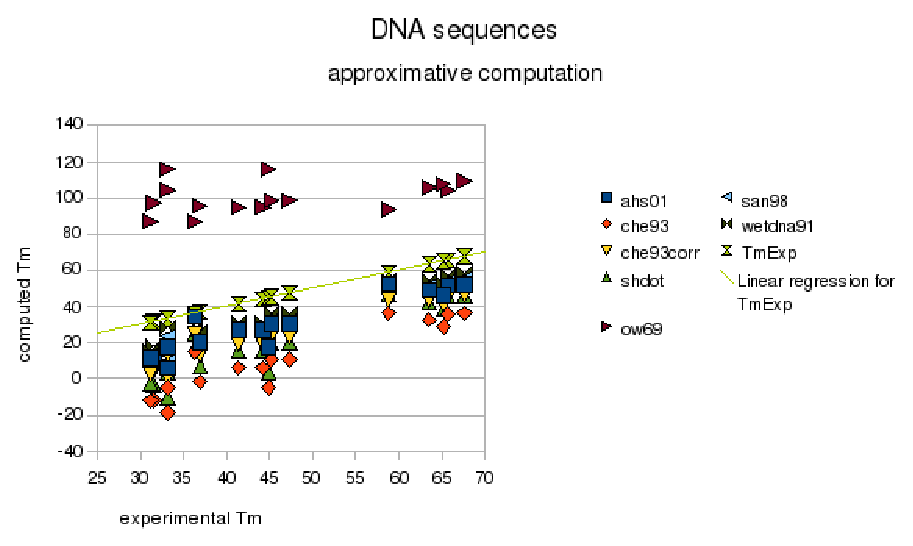
\includegraphics[width=1\linewidth]{images/DNAApproximativeMode}
\caption{Comparison of experimental and computed Tm for various sets of
 DNA approximative formulas. $[\mbox{Na}^+] = 1$~M}
\end{figure}   

\begin{figure}[h]
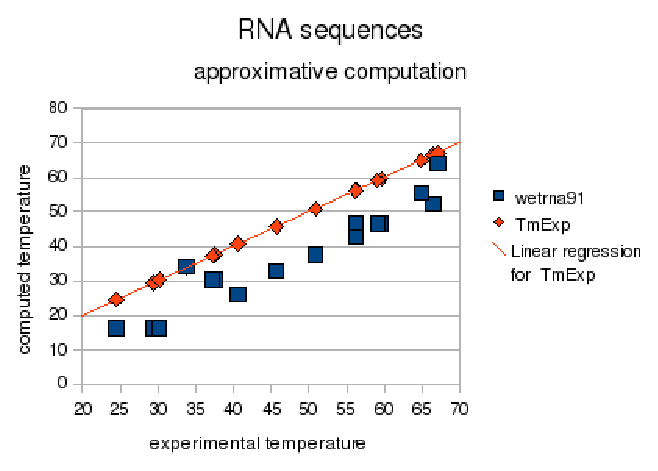
\includegraphics[width=1\linewidth]{images/RNAApproximativeMode}
\caption{Comparison of experimental and computed Tm for various sets of
 RNA approximative formulas. $[\mbox{Na}^+] = 1$~M}
\end{figure}

\begin{figure}[h]
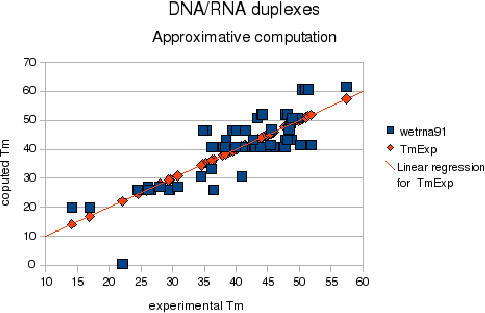
\includegraphics[width=1\linewidth]{images/DNARNAApproximativeMode}
\caption{Comparison of experimental and computed Tm for various sets of
 DNARNA approximative formulas. $[\mbox{Na}^+] = 1$~M, $[\mbox{nucleic acid}] = 4\cdot{}10^{-4}$~M}
\end{figure}      
 
\clearpage
\bibliographystyle{plain}
\bibliography{melting}  
 
\section{See Also }
New versions and 
related material can be found at 

\url{http://www.pasteur.fr/recherche/unites/neubiomol/meltinghome.html} 

\url{https://sourceforge.net/projects/melting/}

\url{http://www.ebi.ac.uk/compneur-srv/melting/}
  
You can use \textsc{melting} through a web server at 
\url{http://bioweb.pasteur.fr/seqanal/interfaces/melting.html}
\url{http://www.ebi.ac.uk/compneur-srv/melting/melt.php}   
   
\section{Copyright }
Melting is copyright 
\copyright 1997, 2009 by Nicolas Le Nov\`ere and Marine Dumousseau.  

This program is free software; 
you can redistribute it and/or modify it under the terms of the GNU General 
Public License as published by the Free Software Foundation; either version 
2 of the License, or (at your option) any later version.   
  This program 
is distributed in the hope that it will be useful, but WITHOUT ANY WARRANTY; 
without even the implied warranty of MERCHANTABILITY or FITNESS FOR A 
PARTICULAR PURPOSE.  See the GNU General Public License for more details. 
  
  You should have received a copy of the GNU General Public License 
along with this program; if not, write to the Free Software Foundation, 
Inc., 59 Temple Place, Suite 330, Boston, MA  02111-1307 USA   
   
\section{Acknowledgements}
Nicolas Joly is an efficient and kind debugger and advisor.  Catherine
Letondal wrote the HTML interface to melting. Thanks to Nirav Merchant,
Taejoon Kwon, Leo Schalkwyk, Mauro Petrillo, Andrew Thompson, Wong Chee Hong, Ivano
Zara for their bug fixes and comments. Thanks to Richard Owczarzy for his magnesium 
correction. Thanks to Charles Plessy for the graphical interface files. Finally thanks
to the usenet helpers, particularly Olivier Dehon and Nicolas Chuche.

   
\section{Authors }
Nicolas Le Nov\`ere and Marine Dumousseau, \\
EMBL-EBI, 
Wellcome-Trust Genome Campus
Hinxton Cambridge, CB10 1SD, UK
lenov@ebi.ac.uk
  
\section{History }

The Java version has been rewriten from the beginning.
See the file ChangeLog for the changes of the versions 4 and more recent.

\end{document}
